\documentclass[11pt]{article}
\usepackage[top = 0.6 in, bottom = 0.6 in, left = 1 in, right = 1 in]{geometry}
\usepackage{graphicx}
% \usepackage{caption2}
\usepackage{anyfontsize}
\usepackage{setspace}
\usepackage{listings}
\usepackage{xcolor}
\usepackage{float}
\usepackage{amsmath}
\usepackage{subcaption}
\usepackage{lineno}

%\usepackage{mwe}



\setlength{\parindent}{0em}
\setlength{\parskip}{1em}
\renewcommand{\baselinestretch}{1.5}

\title{Model Analysis of Biological Temperature-Responsive Rates}
\author{Jingkai Sun (CID: 01991822)}
\date{\today}


\begin{document}


\begin{titlepage}

    \newcommand{\HRule}{\rule{\linewidth}{0.5mm}} % Defines a new command for the horizontal lines, change thickness here
    \newcommand{\wordcount}{\documentclass[11pt]{article}
\usepackage[top = 0.6 in, bottom = 0.6 in, left = 1 in, right = 1 in]{geometry}
\usepackage{graphicx}
% \usepackage{caption2}
\usepackage{anyfontsize}
\usepackage{setspace}
\usepackage{listings}
\usepackage{xcolor}
\usepackage{float}
\usepackage{amsmath}
\usepackage{subcaption}
\usepackage{lineno}

%\usepackage{mwe}



\setlength{\parindent}{0em}
\setlength{\parskip}{1em}
\renewcommand{\baselinestretch}{1.5}

\title{Model Analysis of Biological Temperature-Responsive Rates}
\author{Jingkai Sun (CID: 01991822)}
\date{\today}


\begin{document}


\begin{titlepage}

    \newcommand{\HRule}{\rule{\linewidth}{0.5mm}} % Defines a new command for the horizontal lines, change thickness here
    \newcommand{\wordcount}{\documentclass[11pt]{article}
\usepackage[top = 0.6 in, bottom = 0.6 in, left = 1 in, right = 1 in]{geometry}
\usepackage{graphicx}
% \usepackage{caption2}
\usepackage{anyfontsize}
\usepackage{setspace}
\usepackage{listings}
\usepackage{xcolor}
\usepackage{float}
\usepackage{amsmath}
\usepackage{subcaption}
\usepackage{lineno}

%\usepackage{mwe}



\setlength{\parindent}{0em}
\setlength{\parskip}{1em}
\renewcommand{\baselinestretch}{1.5}

\title{Model Analysis of Biological Temperature-Responsive Rates}
\author{Jingkai Sun (CID: 01991822)}
\date{\today}


\begin{document}


\begin{titlepage}

    \newcommand{\HRule}{\rule{\linewidth}{0.5mm}} % Defines a new command for the horizontal lines, change thickness here
    \newcommand{\wordcount}{\documentclass[11pt]{article}
\usepackage[top = 0.6 in, bottom = 0.6 in, left = 1 in, right = 1 in]{geometry}
\usepackage{graphicx}
% \usepackage{caption2}
\usepackage{anyfontsize}
\usepackage{setspace}
\usepackage{listings}
\usepackage{xcolor}
\usepackage{float}
\usepackage{amsmath}
\usepackage{subcaption}
\usepackage{lineno}

%\usepackage{mwe}



\setlength{\parindent}{0em}
\setlength{\parskip}{1em}
\renewcommand{\baselinestretch}{1.5}

\title{Model Analysis of Biological Temperature-Responsive Rates}
\author{Jingkai Sun (CID: 01991822)}
\date{\today}


\begin{document}


\begin{titlepage}

    \newcommand{\HRule}{\rule{\linewidth}{0.5mm}} % Defines a new command for the horizontal lines, change thickness here
    \newcommand{\wordcount}{\input{TPC_project.sum}} % Supervisor's Name
    
    %----------------------------------------------------------------------------------------
    %	LOGO SECTION
    %----------------------------------------------------------------------------------------
    
    
\includegraphics[width=7cm]{images/logo.eps}\\[1cm] 
    % Include a department/university logo - this will require the graphicx package
     
    %----------------------------------------------------------------------------------------
    
    \center % Center everything on the page
    
    %----------------------------------------------------------------------------------------
    %	HEADING SECTIONS
    %----------------------------------------------------------------------------------------
    
    % \textsc{\LARGE MSc Computational Methods in Ecology and Evolution}\\[1.5cm] % Name of your university/college
    \textbf{\large Imperial College London}\\[0.8 cm] % Major heading such as course name
    \textbf{\large Department of Life Sciences, Faculty of Natural Sciences}\\[0.8 cm] % Minor heading such as course title
    %----------------------------------------------------------------------------------------
    %	TITLE SECTION
    %----------------------------------------------------------------------------------------
    \makeatletter
    \HRule \\[0.6cm]
    { \huge \bfseries \@title}\\[0.6cm] % Title of your document
    \HRule \\[1.5cm]

    \begin{minipage}{0.4\textwidth}
      \begin{flushleft} \large
      \emph{Author:}\\
      Jingkai \textsc{SUN} \\[0.5cm]
      \emph{CID:}\\
      01991822
      \end{flushleft}
      \end{minipage}
      ~
      \begin{minipage}{0.5\textwidth}
      \begin{flushright} \large
      \emph{Date:} \\
      \today \\[0.5cm] % Supervisor's Name
      \emph{Word Count:} \\
      \wordcount


      \end{flushright}
    \end{minipage}\\[1cm]
 
 
    % \center
    % \textbf{\huge Word Count: 2065}
    
    \vfill % Fill the rest of the page with whitespace
    
    \end{titlepage}

\maketitle
\linenumbers

\begin{abstract}
The photosynthesis and respiration rate are essential biological traits of organisms, they are all responsed to their body temperature, indicating that creating effective mathematical model to describe them is becoming increasingly crucial. This project has used four candidate models (Quadratic, Cubic, Briere and simplified Schoolfield models), where quadratic, cubic and briere are phenomenological models and simplified Schoolfield is mechanistic model, to fit 378 datasets of photosynthesis rate and 249 datasets of respiration rate grouped by different IDs of organisms. The result shows that simplified Schoolfield model is effective for fitting datasets of photosynthesis rate, although cubic may be better than it in some cases.
\end{abstract}


\section{Introduction}

Thermal performance curve (TPC) describes the relationship between biological traits (e.g. photosynthesis, respiration and growth rate) and temperature, which is an essential factor in ecology, biology and physiology \cite{huey_1989}. Due to the importance of TPC, numerous biological temperature-dependent rate models have been implemented, it has been increasingly important that using computer tools to fit the model \cite{angilletta_2002}, many authors have taken advantages of programming language for model fitting in their paper. However, the paper concerning the comparison between published models is scarce. Therefore, this project aims at giving a comparison between distinct models fitting the thermal performance curve. The remaining sections in this report will be explained as follow. In section 2, a brief introduction of candidate models and an explanation of data preprocessing will be given, then I will explain the method and assessment tool used. In section 3, the results of the fitted model will be explained. Next section will give a conclusion for the results and some future works that can be done.

\section{Experimental Data and Fitting Methods}

\subsection{Experimental Data}

The part of ”BioTraits” database, containing 903 fitted subsets, was selected as the main research object for the model analysis with columns (”ID”, ”ConTemp(°C)”, ”OriginalTraitValue”, ”StandardisedTraitName”). Some preprocess had been done to the original dataset. Firstly, all observations where the Original Trait Value is less than or equal to zero had been removed for logarithm purpose. Then, to obtain more reasonable curves, all datasets in which data points are less than or equal to 5 (276 out of 903) were deleted. Afterwards, the datasets were divided into two subsets based on the ”StandardisedTraitName”, which is ”photosynthesis rate” and ”respiration rate”. Then, there were 378 and 249 (627 subsets in total) subsets in two datasets with different biological traits respectively.

\subsection{Candidate Models}

Four models were chosen in this project, including two linear models (Quadratic and Cubic) and two non-linear models (Briere and Schoolfield Model with High-Temperature Term). For two linear and Briere models, they are phenomenological models lacking some biological interpretation, while Schoolfield is a mechanistic model that has some biological meaning behind that. Briere (1) and Schoolfield (2) model have mathematical expressions as follow:

\begin{equation}
    B =
    \begin{cases}
    0,                           &\text{$T \leq T_0$} \\
    B_0T(T-T_0) \sqrt {T_m - T}, &\text{$T_0 \leq T \leq T_m$} \\
    0,                           &\text{$T \geq T_m$}
    \end{cases}
\end{equation}

where B is biological trait, which is a function of temperature T. $T_l$ is the maximum temperature that organisms can bear.
$T_0$ is the lowest temperature threshold, and B0 is the empirical constant. There are some assumptions for fitting the data well \cite{briere_pracros_1999}.

\begin{itemize}
    \item It is possible to adjust the muximum or minimum thresholds of temperature \cite{briere_pracros_1999}. 
    \item Asymmetric shape around peak temperature ($T_{opt}$) \cite{briere_pracros_1999}.
    \item There is a sharp drop after passing the $T_{opt}$ \cite{briere_pracros_1999}.
    \item There is an inflection point in the datasets \cite{briere_pracros_1999}.
\end{itemize}

The full Schoolfield model is expressed as follows \cite{SCHOOLFIELD1981719}:
\begin{equation}
    B = B_0 \frac { e^{\frac{-E_a}{k}(\frac{1}{T} - \frac{1}{283.5})} }
                { 1 + e^{\frac{E_l}{k}(\frac{1}{T_l} - \frac{1}{T})} + 
                e^{\frac{E_h}{k} (\frac{1}{T_h} - \frac{1}{T}) }}
\end{equation}

where k is Boltzmann constant, B is the biological rate responsed by temperature T in Kelvin unit. $B_0$ is the biological rate at low temperature. $E_a$ is the activation energy that determine the increase in temperature up to the optimum. $E_l$ 
is the de-activation energy at low temperature. $T_l$ is the low temperature that enzyme is 50\% de-activated. $E_h$ is the de-activation energy at high temperature, while $T_h$ is temperature at which the enzyme is 50\% high-temperature deactivated.
However, it is difficult to detect the low-temperature deactivation energy \cite{kontopoulos_2018}. Thus, the schoolfield with only high temperature term (eq.3) was used in this porject:

\begin{equation}
    B = B_0 \frac { e^{\frac{-E_a}{k}(\frac{1}{T} - \frac{1}{283.5})} }
                { 1 + e^{\frac{E_h}{k} (\frac{1}{T_h} - \frac{1}{T}) }}
\end{equation}

To capture the data pattern more precisely, the Schoolfield equation is rewritten as logarithmic form:

\begin{equation}
    ln(B) = ln(B_0) - \frac{E_a}{k} \times (\frac{1}{T} - \frac{1}{283.5}) - ln(1 + e^{\frac{E_h}{k} (\frac{1}{T_h} - \frac{1}{T}) })
\end{equation}

With simplified Schoolfield model, some assumptions are also needed to capture the data pattern well \cite{delong_2017}:

\begin{itemize}
    \item All traits (biological rates) is controlled by single enzyme \cite{delong_2017}
    \item enzymes need to be deactivated at high temperature \cite{delong_2017}
    \item the activation energy ($E_a$) corresponds to the optimal enzyme activity level \cite{delong_2017}
\end{itemize}

In addition, this project also assumes that there is no interation terms between linear models.

\subsection{Model Assessment}

All four candidate models mentioned above were assessed. The starting values of two non-linear models were found as follow:
For Briere model, the maximum and minimum temperature is given by parameters $T_m$ and $T_0$ respectively. Initial $B_0$ is chosen to be 0.01 manually. For simplified Schoolfield model, initial $B_0$ is just the biological rate at the lowest temperature. $E_a$ and  $E_h$ are selected to be the absolute values of slope and slope times ten by running the logarithmic Arrhenius model respectively.  Finally, the temperature (or the average of the temperature if there more than two values) that has the highest rate is given to the initial $T_h$. After assigning initial values, the starting value will be chosen randomly using normal distribution method with mean as the value of parameters as well as appropriate bounding and standard deviation values, the fitted data such as TSS, RSS, $R^2$, AIC and BIC are calculated. The whole fitting process will be repeated by a minimum 200 and maximum of 300 rounds in order to find the best fit with the lowest AIC value.

Akaike Information Criterion (AIC) and Bayesian Information Criterion (BIC) were calculated for model analysis. These metrics allow us to choose which model performs the best. The AIC approach is an information-theoretic selection by calculating Kullback-Leibler (K-L) distance \cite{burnham_anderson_2004} \cite{burnham_anderson2010}, while the BIC method is based on Bayes factors. All those values are expected to be the lower, the better. However, these metrics will cause the issue if they are used independently since they are used to compare with other values, there is no point computing AIC vlaue for single model. \cite{guthery_2003}. Thus, the AIC differences were also calculated in order to rank models and include more reasonable best-fit models. The rule of thumb of AIC differences allows us to consider more models as the best-fit model for each trial if the value differences between two models are less than 2, expressed as $ \Delta AIC_i/BIC_i < 2$ \cite{burnham_anderson2010}.


\subsection{Computing Tools}

In this project, Python 3 with packages "lmfit", "numpy", "pandas" and "matplotlib" was used as the main tool of creating model fitting program. R (4.0.3) with packages "dplyr" and "ggplot2" was used to analyse and visualise the fitted information of each model obtained after the model fitting program is done. Python 3 with package "subprocess" and "os" was used to integrate all project scripts.

\section{Results}
% Figures of total counts
\begin{figure}[H]
    \centering
    \includegraphics[width = 15cm, height = 12cm]{images/bestfit_total_rule2.pdf}
    \caption{Best fit occurrence using rule of $\Delta AIC/BIC + 2$}
\end{figure}

Figure 1 gives the best-fit occurrence for each models using AIC or BIC difference rule. Surprisingly, cubic has the most outstanding performance compared with all other models. However, simplified Schoolfield, the only mechanistic model in candidate ones, has the second most times becoming the best fit model. Cubic is the best model of 387 datasets (based on AIC assessment) and 337 datasets (based on BIC assessment) out of 627 datasets, accounting for approximately 67\% and 58\% of total datasets respectively, while simplified Schoolfield is the best model of 245 and 237 datasets based on different measurement metrics, accounting for 42\% and 41\% of the total. Also, 108 datasets have both cubic and Schoolfield models as best fit models based on the rule of AIC/BIC differences. For the remaining two models, quadratic became the best-fit model of 198 and 201 datasets according to AIC and BIC values, which is 34 and 33 datasets more than Briere. 

\begin{figure}[H]
    % \hspace*{-1cm}
    \center
    \includegraphics[height = 14cm, width = 15cm]{images/bestfit_grouped_rule2.pdf}
    \caption{Best-Fit Occurence Based on Different Datasets and Assessment Methods}
\end{figure}

Figure 2 illustrates the number of best-fit models in datasets of photosynthesis and respiration rate using AIC or BIC difference and the method of single model selection with the lowest AIC/BIC values. First of all, with using the AIC/BIC difference approach to count best models, two datasets showed very different results. For the dataset of photosynthesis, furthermore, cubic and simplified Schoolfield are also the top 2 models that have the highest counts of the best fit. Cubic is the best-fit model of 191 datasets of fitting out of 335 datasets, which is 29 datasets more than the simplified Schoolfield using AIC approach but only 7 more by BIC approach, while there is no significant difference between quadratic and Briere models. In respiration datasets, cubic is still the winner compared other models, becoming the best-fit model in 81\% or 70\% of the total by distinct model assessment approaches. However, quadratic became the second best-fit model, taking the place of the simplified Schoolfield model. By choosing the single model with lowest AIC/BIC values in each trial, interestingly, the simplified Schoolfield model beats all other three models, being the best model in 35\% - 36\% of total photosynthesis data, while cubic and quadratic models still outperform other ones in the dataset of respiration rate.

\section{Discussion}

\begin{figure}
    \begin{subfigure}[t]{.5\textwidth}
      \center
      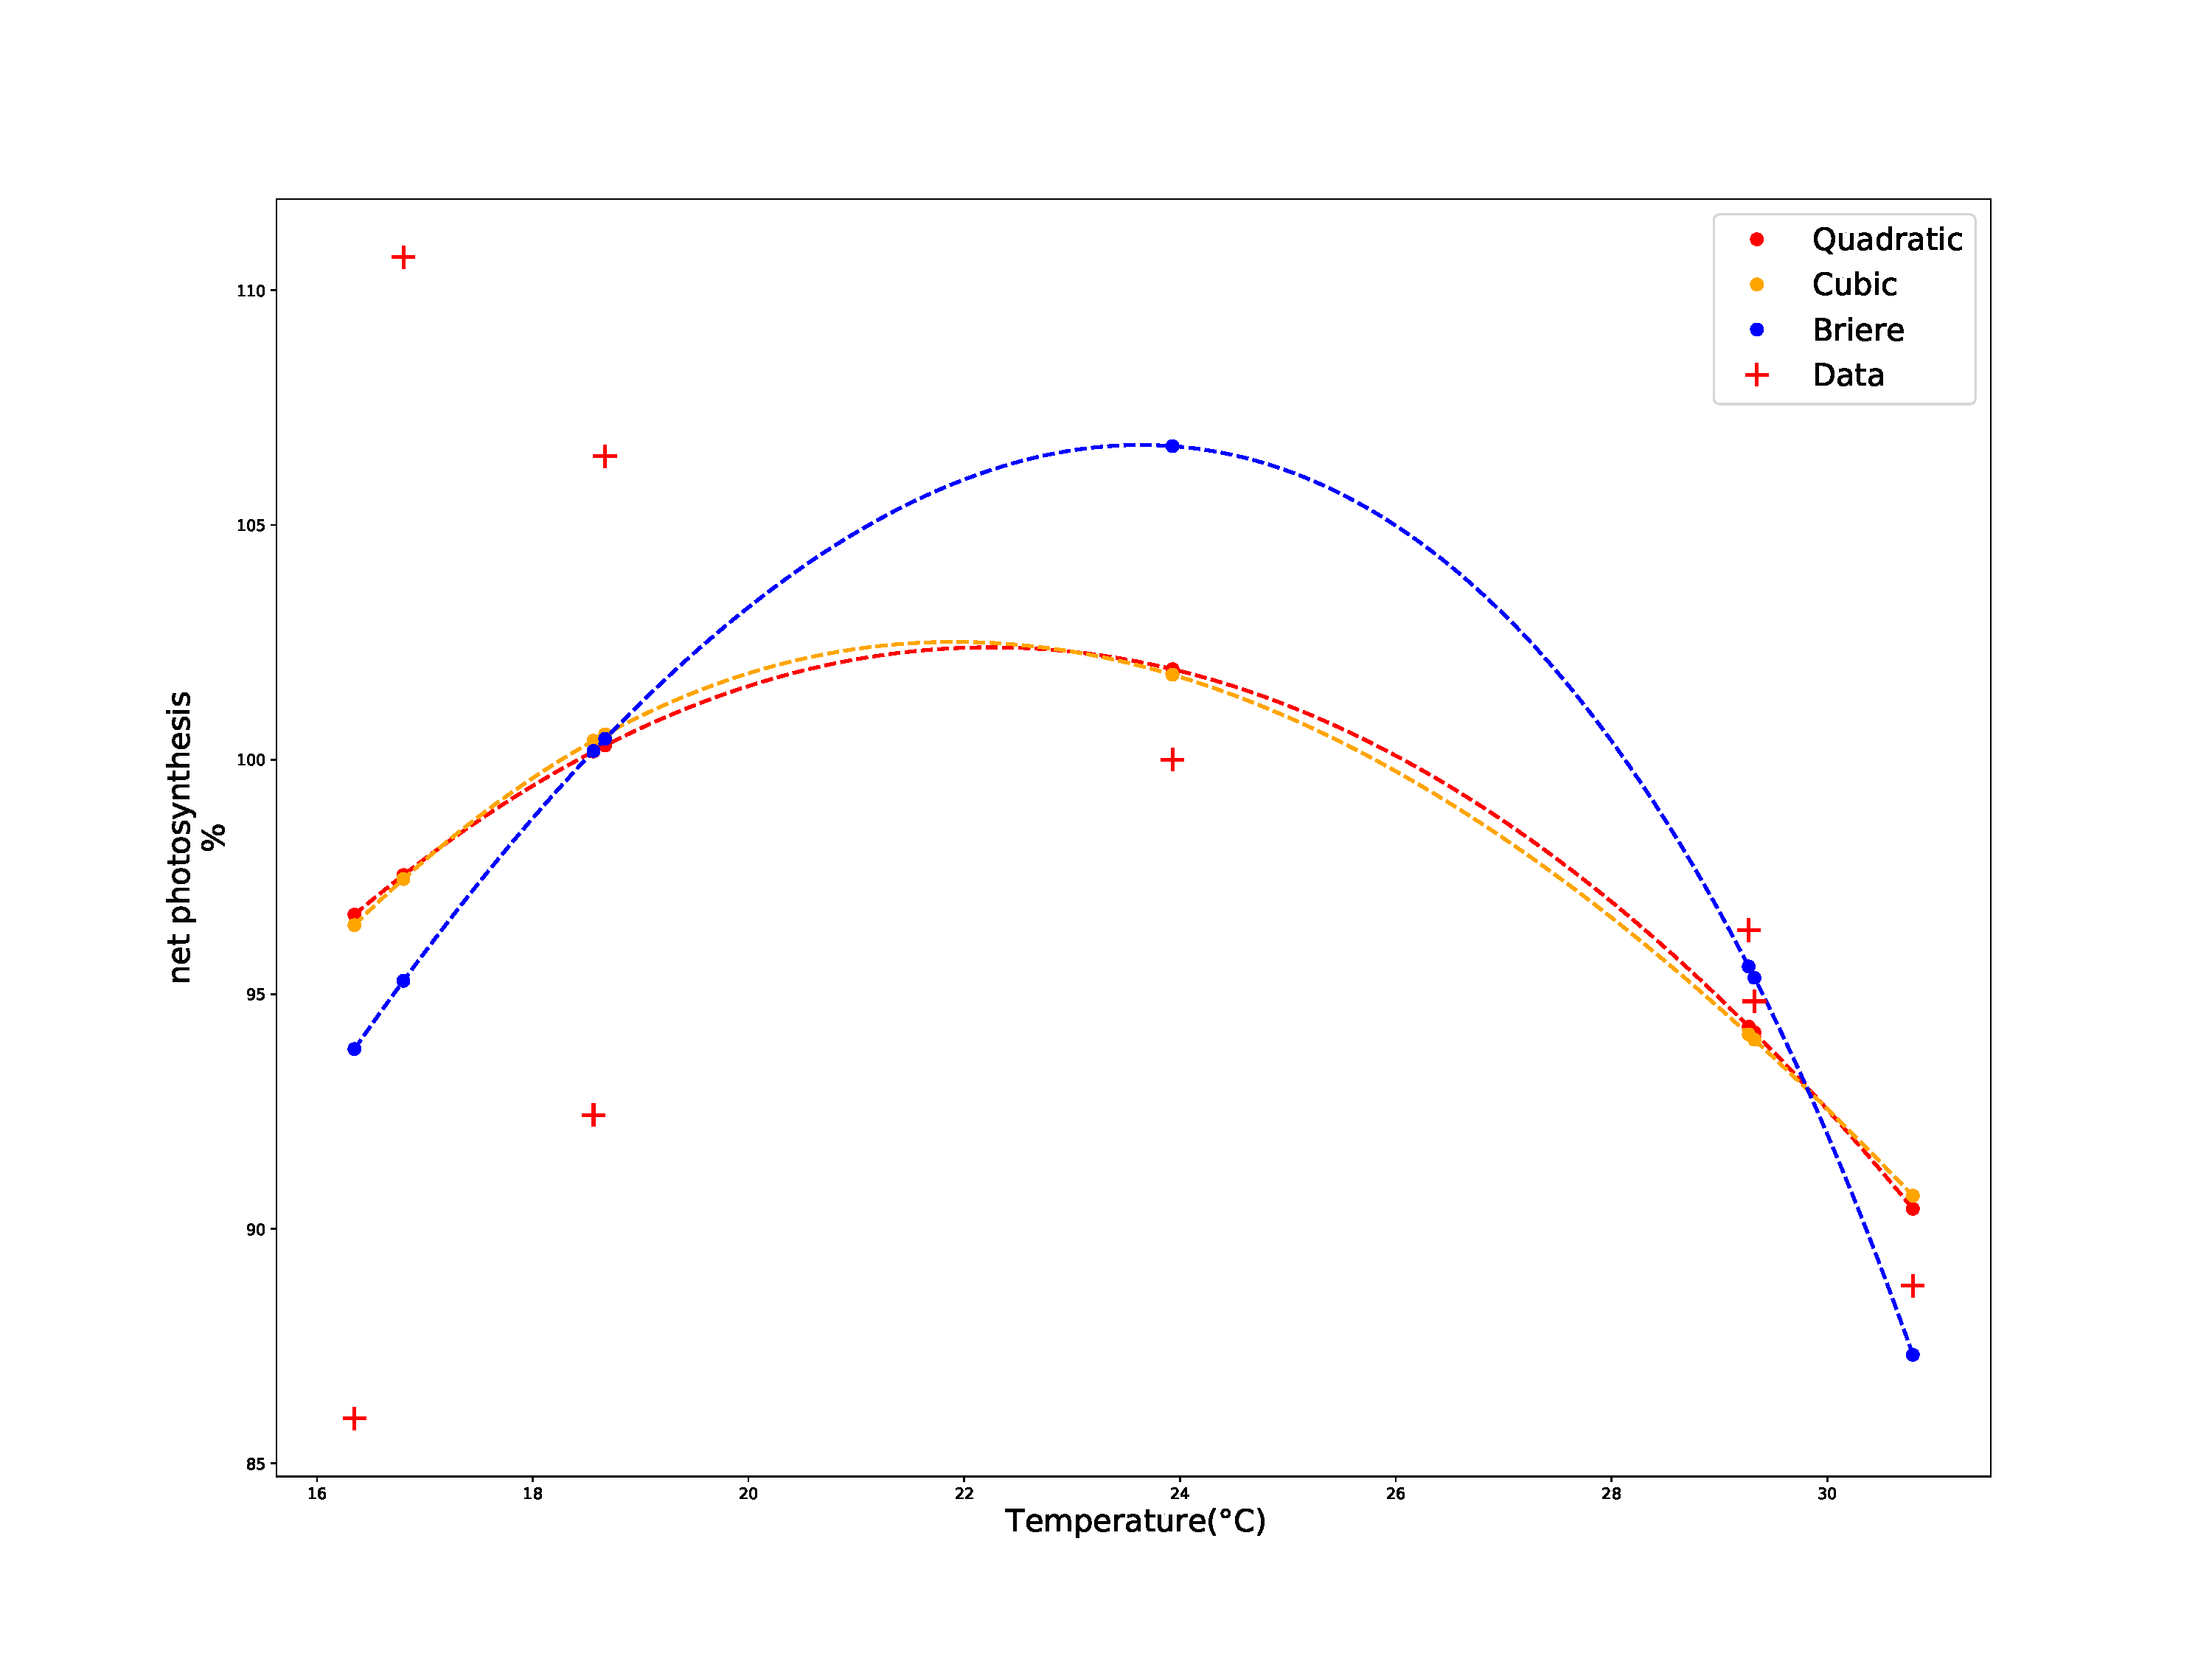
\includegraphics[width=\linewidth]{images/TPC_fitting511.pdf}
      \caption{\textbf{ID:511}}
    \end{subfigure}
    \hfill
    \begin{subfigure}[t]{.5\textwidth}
      \center
      \includegraphics[width=\linewidth]{images/TPC_fitting519.pdf}
      \caption{\textbf{ID:519}}
    \end{subfigure}
  
    \medskip

  % \hspace*{-1cm}
    \begin{subfigure}[t]{.5\textwidth}
      \center
      \includegraphics[width=\linewidth]{images/TPC_fitting568.pdf}
      \caption{\textbf{ID: 568}}
    \end{subfigure}
    \hfill
    \begin{subfigure}[t]{.5\textwidth}
    \center
      \includegraphics[width=\linewidth]{images/TPC_fitting600.pdf}
      \caption{\textbf{ID: 600}}
    \end{subfigure}
    \caption{Datasets that have poor fitting of mechanistic model}
  \end{figure}

  From the results shown above, there is no significant difference in model assessment between the AIC approach and BIC approach. The rank of the best-fit model is not affected, although a little gap can be seen for each model as different approaches of model assessment apply.  Also, the trend is similar to the most datasets when distinct rules apply except for the dataset of photosynthesis, where a significant differences between model performance of cubic model can be seen as applying different rules.

  Due to the interpretability of the mechanistic model, it is expected to be have better performance than some phenomenological or statistical models. However, it is not always true in the project, where the simplified Schoolfield model was the best model only in the photosynthesis dataset when applying rule of single model selection. The reason for this may the mechanistic models have more restrict hypotheses than phenomenological ones, which results in the fitting of mechanistic model is invalid. The figure 3 showed some examples of failed or poor fittings of individual datasets. 

  By comparison, AIC and BIC both provided similar outcomes and model selection, although there may be a little differences between results of them. Thus, any one of them can be selected as a main model assessment method in my project. However, AIC was preferred to use in this project. The reasion is (1) AIC is a suitable approach for sparse datasets, given that it is an estimator derived from basic thoery called K-L information theory, which is possible for further correction.Thus, this leads AIC to have second-order derived version that can deliminate estimated bias of small sample size \cite{burnham_anderson_2004}. (2) BIC expects the "true model" to be in the model set while AIC does not \cite{johnson_2004}.

  The motivation of the project is to analyse four candidate models and provide a reasonable comparison between them. However, there are also more works need to be done. Firstly, the starting values of two non-linear models are selected by normal distribution sampling method, which may be not enough for finding the precise starting values. Thus, this may be also the reason why linear model outperformed non-linear model in respiration dataset. A better approach to find the starting value of parameters for non-linear models should be implemented. Secondly, only one mechanistic model are used to make a model comparison here, may causing bias of the results. Thus, more mechanistic models are worthy of consideration in order to improve the accuracy of the results. Third, due to limited computational power, only approximately maximum 300 repeats of fitting for each indivial dataset is available. Hence, more repeats are suppose to be attempted for obtaining more accurate outcome if the computer with stronger computational power is available such as high-performance computer or other supercomputers.

\section{Conclusion}

In conclusion, the mechanistic model, simplified Schoolfield, is significantly useful when fitting the data of biological rate since the data pattern of approximately 42\% of dataset was captured, although cubic model outperformed it in some cases. However, the simplified Schoolfield model does not show an obvious advantage when fitting the datasets of respiration rate, due to the data specificity and strictness of assumptions of mechanistic models. Therefore, there is no sufficient evidence that can conclude that mechanistic model is better than phenomenological models. To select the best models between them, if possible, all datasets should be considered case by case.

\bibliographystyle{plain}
\bibliography{references}


% \section{Appendices}
\end{document}} % Supervisor's Name
    
    %----------------------------------------------------------------------------------------
    %	LOGO SECTION
    %----------------------------------------------------------------------------------------
    
    
\includegraphics[width=7cm]{images/logo.eps}\\[1cm] 
    % Include a department/university logo - this will require the graphicx package
     
    %----------------------------------------------------------------------------------------
    
    \center % Center everything on the page
    
    %----------------------------------------------------------------------------------------
    %	HEADING SECTIONS
    %----------------------------------------------------------------------------------------
    
    % \textsc{\LARGE MSc Computational Methods in Ecology and Evolution}\\[1.5cm] % Name of your university/college
    \textbf{\large Imperial College London}\\[0.8 cm] % Major heading such as course name
    \textbf{\large Department of Life Sciences, Faculty of Natural Sciences}\\[0.8 cm] % Minor heading such as course title
    %----------------------------------------------------------------------------------------
    %	TITLE SECTION
    %----------------------------------------------------------------------------------------
    \makeatletter
    \HRule \\[0.6cm]
    { \huge \bfseries \@title}\\[0.6cm] % Title of your document
    \HRule \\[1.5cm]

    \begin{minipage}{0.4\textwidth}
      \begin{flushleft} \large
      \emph{Author:}\\
      Jingkai \textsc{SUN} \\[0.5cm]
      \emph{CID:}\\
      01991822
      \end{flushleft}
      \end{minipage}
      ~
      \begin{minipage}{0.5\textwidth}
      \begin{flushright} \large
      \emph{Date:} \\
      \today \\[0.5cm] % Supervisor's Name
      \emph{Word Count:} \\
      \wordcount


      \end{flushright}
    \end{minipage}\\[1cm]
 
 
    % \center
    % \textbf{\huge Word Count: 2065}
    
    \vfill % Fill the rest of the page with whitespace
    
    \end{titlepage}

\maketitle
\linenumbers

\begin{abstract}
The photosynthesis and respiration rate are essential biological traits of organisms, they are all responsed to their body temperature, indicating that creating effective mathematical model to describe them is becoming increasingly crucial. This project has used four candidate models (Quadratic, Cubic, Briere and simplified Schoolfield models), where quadratic, cubic and briere are phenomenological models and simplified Schoolfield is mechanistic model, to fit 378 datasets of photosynthesis rate and 249 datasets of respiration rate grouped by different IDs of organisms. The result shows that simplified Schoolfield model is effective for fitting datasets of photosynthesis rate, although cubic may be better than it in some cases.
\end{abstract}


\section{Introduction}

Thermal performance curve (TPC) describes the relationship between biological traits (e.g. photosynthesis, respiration and growth rate) and temperature, which is an essential factor in ecology, biology and physiology \cite{huey_1989}. Due to the importance of TPC, numerous biological temperature-dependent rate models have been implemented, it has been increasingly important that using computer tools to fit the model \cite{angilletta_2002}, many authors have taken advantages of programming language for model fitting in their paper. However, the paper concerning the comparison between published models is scarce. Therefore, this project aims at giving a comparison between distinct models fitting the thermal performance curve. The remaining sections in this report will be explained as follow. In section 2, a brief introduction of candidate models and an explanation of data preprocessing will be given, then I will explain the method and assessment tool used. In section 3, the results of the fitted model will be explained. Next section will give a conclusion for the results and some future works that can be done.

\section{Experimental Data and Fitting Methods}

\subsection{Experimental Data}

The part of ”BioTraits” database, containing 903 fitted subsets, was selected as the main research object for the model analysis with columns (”ID”, ”ConTemp(°C)”, ”OriginalTraitValue”, ”StandardisedTraitName”). Some preprocess had been done to the original dataset. Firstly, all observations where the Original Trait Value is less than or equal to zero had been removed for logarithm purpose. Then, to obtain more reasonable curves, all datasets in which data points are less than or equal to 5 (276 out of 903) were deleted. Afterwards, the datasets were divided into two subsets based on the ”StandardisedTraitName”, which is ”photosynthesis rate” and ”respiration rate”. Then, there were 378 and 249 (627 subsets in total) subsets in two datasets with different biological traits respectively.

\subsection{Candidate Models}

Four models were chosen in this project, including two linear models (Quadratic and Cubic) and two non-linear models (Briere and Schoolfield Model with High-Temperature Term). For two linear and Briere models, they are phenomenological models lacking some biological interpretation, while Schoolfield is a mechanistic model that has some biological meaning behind that. Briere (1) and Schoolfield (2) model have mathematical expressions as follow:

\begin{equation}
    B =
    \begin{cases}
    0,                           &\text{$T \leq T_0$} \\
    B_0T(T-T_0) \sqrt {T_m - T}, &\text{$T_0 \leq T \leq T_m$} \\
    0,                           &\text{$T \geq T_m$}
    \end{cases}
\end{equation}

where B is biological trait, which is a function of temperature T. $T_l$ is the maximum temperature that organisms can bear.
$T_0$ is the lowest temperature threshold, and B0 is the empirical constant. There are some assumptions for fitting the data well \cite{briere_pracros_1999}.

\begin{itemize}
    \item It is possible to adjust the muximum or minimum thresholds of temperature \cite{briere_pracros_1999}. 
    \item Asymmetric shape around peak temperature ($T_{opt}$) \cite{briere_pracros_1999}.
    \item There is a sharp drop after passing the $T_{opt}$ \cite{briere_pracros_1999}.
    \item There is an inflection point in the datasets \cite{briere_pracros_1999}.
\end{itemize}

The full Schoolfield model is expressed as follows \cite{SCHOOLFIELD1981719}:
\begin{equation}
    B = B_0 \frac { e^{\frac{-E_a}{k}(\frac{1}{T} - \frac{1}{283.5})} }
                { 1 + e^{\frac{E_l}{k}(\frac{1}{T_l} - \frac{1}{T})} + 
                e^{\frac{E_h}{k} (\frac{1}{T_h} - \frac{1}{T}) }}
\end{equation}

where k is Boltzmann constant, B is the biological rate responsed by temperature T in Kelvin unit. $B_0$ is the biological rate at low temperature. $E_a$ is the activation energy that determine the increase in temperature up to the optimum. $E_l$ 
is the de-activation energy at low temperature. $T_l$ is the low temperature that enzyme is 50\% de-activated. $E_h$ is the de-activation energy at high temperature, while $T_h$ is temperature at which the enzyme is 50\% high-temperature deactivated.
However, it is difficult to detect the low-temperature deactivation energy \cite{kontopoulos_2018}. Thus, the schoolfield with only high temperature term (eq.3) was used in this porject:

\begin{equation}
    B = B_0 \frac { e^{\frac{-E_a}{k}(\frac{1}{T} - \frac{1}{283.5})} }
                { 1 + e^{\frac{E_h}{k} (\frac{1}{T_h} - \frac{1}{T}) }}
\end{equation}

To capture the data pattern more precisely, the Schoolfield equation is rewritten as logarithmic form:

\begin{equation}
    ln(B) = ln(B_0) - \frac{E_a}{k} \times (\frac{1}{T} - \frac{1}{283.5}) - ln(1 + e^{\frac{E_h}{k} (\frac{1}{T_h} - \frac{1}{T}) })
\end{equation}

With simplified Schoolfield model, some assumptions are also needed to capture the data pattern well \cite{delong_2017}:

\begin{itemize}
    \item All traits (biological rates) is controlled by single enzyme \cite{delong_2017}
    \item enzymes need to be deactivated at high temperature \cite{delong_2017}
    \item the activation energy ($E_a$) corresponds to the optimal enzyme activity level \cite{delong_2017}
\end{itemize}

In addition, this project also assumes that there is no interation terms between linear models.

\subsection{Model Assessment}

All four candidate models mentioned above were assessed. The starting values of two non-linear models were found as follow:
For Briere model, the maximum and minimum temperature is given by parameters $T_m$ and $T_0$ respectively. Initial $B_0$ is chosen to be 0.01 manually. For simplified Schoolfield model, initial $B_0$ is just the biological rate at the lowest temperature. $E_a$ and  $E_h$ are selected to be the absolute values of slope and slope times ten by running the logarithmic Arrhenius model respectively.  Finally, the temperature (or the average of the temperature if there more than two values) that has the highest rate is given to the initial $T_h$. After assigning initial values, the starting value will be chosen randomly using normal distribution method with mean as the value of parameters as well as appropriate bounding and standard deviation values, the fitted data such as TSS, RSS, $R^2$, AIC and BIC are calculated. The whole fitting process will be repeated by a minimum 200 and maximum of 300 rounds in order to find the best fit with the lowest AIC value.

Akaike Information Criterion (AIC) and Bayesian Information Criterion (BIC) were calculated for model analysis. These metrics allow us to choose which model performs the best. The AIC approach is an information-theoretic selection by calculating Kullback-Leibler (K-L) distance \cite{burnham_anderson_2004} \cite{burnham_anderson2010}, while the BIC method is based on Bayes factors. All those values are expected to be the lower, the better. However, these metrics will cause the issue if they are used independently since they are used to compare with other values, there is no point computing AIC vlaue for single model. \cite{guthery_2003}. Thus, the AIC differences were also calculated in order to rank models and include more reasonable best-fit models. The rule of thumb of AIC differences allows us to consider more models as the best-fit model for each trial if the value differences between two models are less than 2, expressed as $ \Delta AIC_i/BIC_i < 2$ \cite{burnham_anderson2010}.


\subsection{Computing Tools}

In this project, Python 3 with packages "lmfit", "numpy", "pandas" and "matplotlib" was used as the main tool of creating model fitting program. R (4.0.3) with packages "dplyr" and "ggplot2" was used to analyse and visualise the fitted information of each model obtained after the model fitting program is done. Python 3 with package "subprocess" and "os" was used to integrate all project scripts.

\section{Results}
% Figures of total counts
\begin{figure}[H]
    \centering
    \includegraphics[width = 15cm, height = 12cm]{images/bestfit_total_rule2.pdf}
    \caption{Best fit occurrence using rule of $\Delta AIC/BIC + 2$}
\end{figure}

Figure 1 gives the best-fit occurrence for each models using AIC or BIC difference rule. Surprisingly, cubic has the most outstanding performance compared with all other models. However, simplified Schoolfield, the only mechanistic model in candidate ones, has the second most times becoming the best fit model. Cubic is the best model of 387 datasets (based on AIC assessment) and 337 datasets (based on BIC assessment) out of 627 datasets, accounting for approximately 67\% and 58\% of total datasets respectively, while simplified Schoolfield is the best model of 245 and 237 datasets based on different measurement metrics, accounting for 42\% and 41\% of the total. Also, 108 datasets have both cubic and Schoolfield models as best fit models based on the rule of AIC/BIC differences. For the remaining two models, quadratic became the best-fit model of 198 and 201 datasets according to AIC and BIC values, which is 34 and 33 datasets more than Briere. 

\begin{figure}[H]
    % \hspace*{-1cm}
    \center
    \includegraphics[height = 14cm, width = 15cm]{images/bestfit_grouped_rule2.pdf}
    \caption{Best-Fit Occurence Based on Different Datasets and Assessment Methods}
\end{figure}

Figure 2 illustrates the number of best-fit models in datasets of photosynthesis and respiration rate using AIC or BIC difference and the method of single model selection with the lowest AIC/BIC values. First of all, with using the AIC/BIC difference approach to count best models, two datasets showed very different results. For the dataset of photosynthesis, furthermore, cubic and simplified Schoolfield are also the top 2 models that have the highest counts of the best fit. Cubic is the best-fit model of 191 datasets of fitting out of 335 datasets, which is 29 datasets more than the simplified Schoolfield using AIC approach but only 7 more by BIC approach, while there is no significant difference between quadratic and Briere models. In respiration datasets, cubic is still the winner compared other models, becoming the best-fit model in 81\% or 70\% of the total by distinct model assessment approaches. However, quadratic became the second best-fit model, taking the place of the simplified Schoolfield model. By choosing the single model with lowest AIC/BIC values in each trial, interestingly, the simplified Schoolfield model beats all other three models, being the best model in 35\% - 36\% of total photosynthesis data, while cubic and quadratic models still outperform other ones in the dataset of respiration rate.

\section{Discussion}

\begin{figure}
    \begin{subfigure}[t]{.5\textwidth}
      \center
      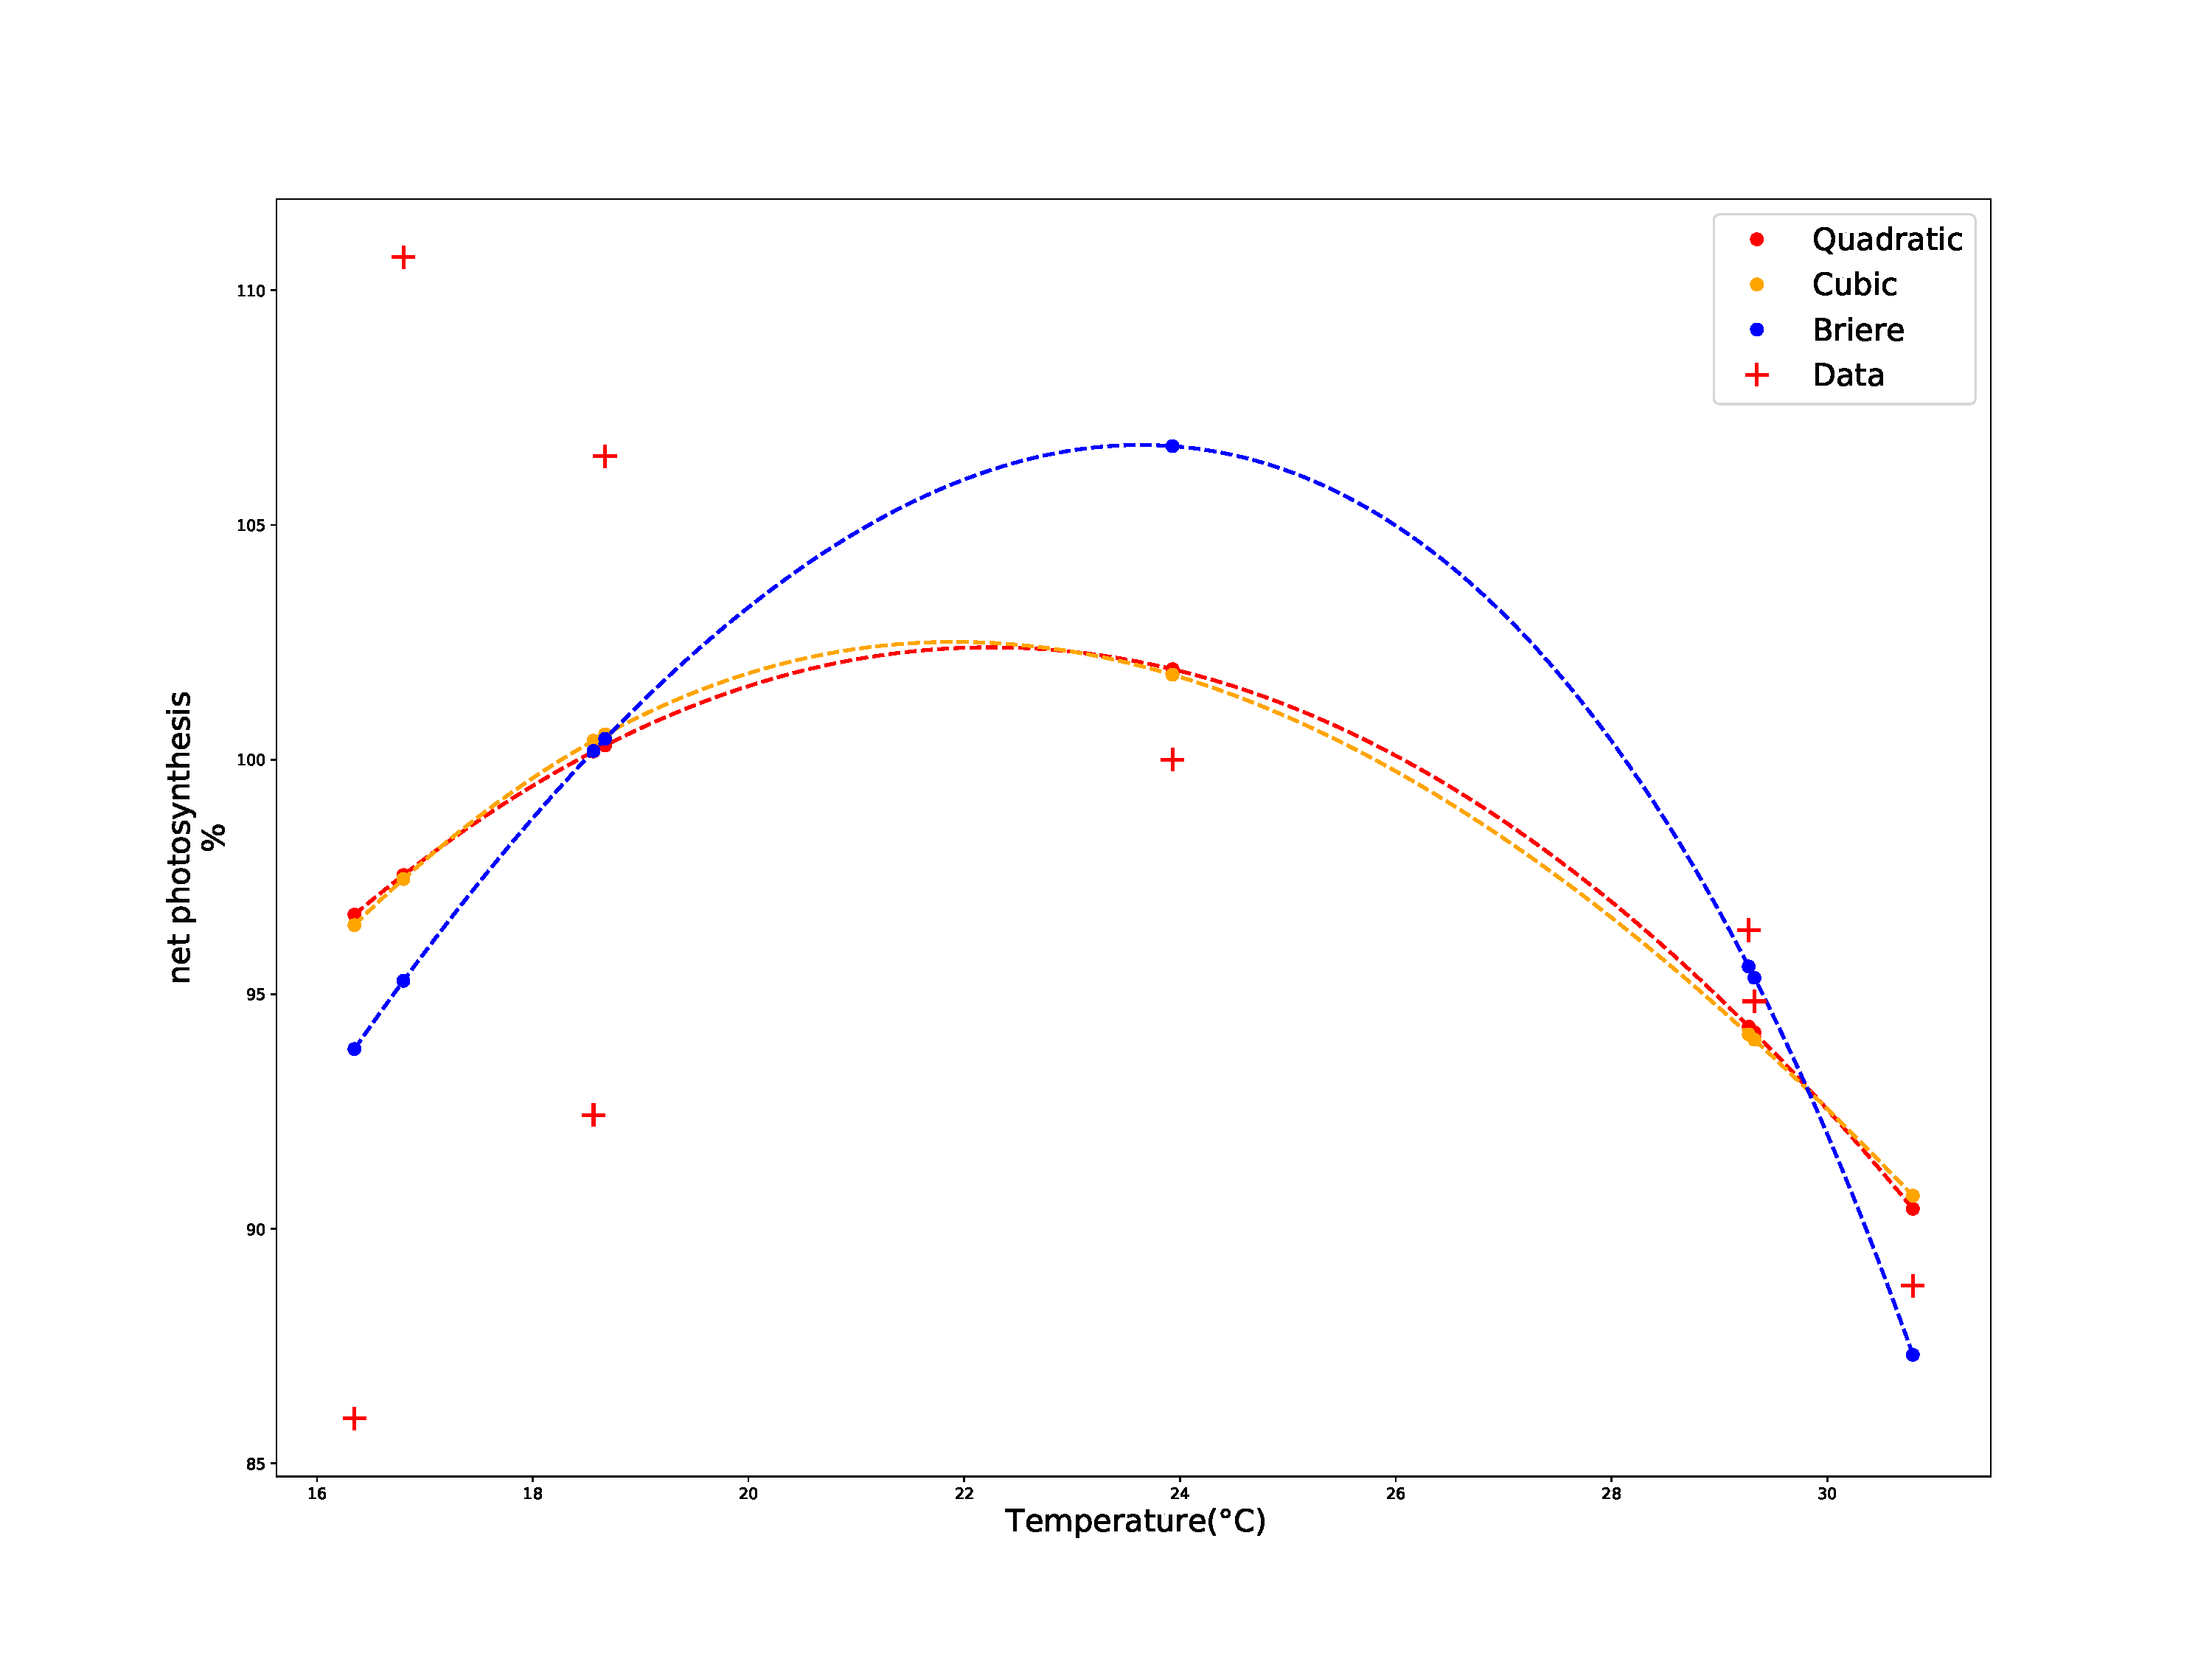
\includegraphics[width=\linewidth]{images/TPC_fitting511.pdf}
      \caption{\textbf{ID:511}}
    \end{subfigure}
    \hfill
    \begin{subfigure}[t]{.5\textwidth}
      \center
      \includegraphics[width=\linewidth]{images/TPC_fitting519.pdf}
      \caption{\textbf{ID:519}}
    \end{subfigure}
  
    \medskip

  % \hspace*{-1cm}
    \begin{subfigure}[t]{.5\textwidth}
      \center
      \includegraphics[width=\linewidth]{images/TPC_fitting568.pdf}
      \caption{\textbf{ID: 568}}
    \end{subfigure}
    \hfill
    \begin{subfigure}[t]{.5\textwidth}
    \center
      \includegraphics[width=\linewidth]{images/TPC_fitting600.pdf}
      \caption{\textbf{ID: 600}}
    \end{subfigure}
    \caption{Datasets that have poor fitting of mechanistic model}
  \end{figure}

  From the results shown above, there is no significant difference in model assessment between the AIC approach and BIC approach. The rank of the best-fit model is not affected, although a little gap can be seen for each model as different approaches of model assessment apply.  Also, the trend is similar to the most datasets when distinct rules apply except for the dataset of photosynthesis, where a significant differences between model performance of cubic model can be seen as applying different rules.

  Due to the interpretability of the mechanistic model, it is expected to be have better performance than some phenomenological or statistical models. However, it is not always true in the project, where the simplified Schoolfield model was the best model only in the photosynthesis dataset when applying rule of single model selection. The reason for this may the mechanistic models have more restrict hypotheses than phenomenological ones, which results in the fitting of mechanistic model is invalid. The figure 3 showed some examples of failed or poor fittings of individual datasets. 

  By comparison, AIC and BIC both provided similar outcomes and model selection, although there may be a little differences between results of them. Thus, any one of them can be selected as a main model assessment method in my project. However, AIC was preferred to use in this project. The reasion is (1) AIC is a suitable approach for sparse datasets, given that it is an estimator derived from basic thoery called K-L information theory, which is possible for further correction.Thus, this leads AIC to have second-order derived version that can deliminate estimated bias of small sample size \cite{burnham_anderson_2004}. (2) BIC expects the "true model" to be in the model set while AIC does not \cite{johnson_2004}.

  The motivation of the project is to analyse four candidate models and provide a reasonable comparison between them. However, there are also more works need to be done. Firstly, the starting values of two non-linear models are selected by normal distribution sampling method, which may be not enough for finding the precise starting values. Thus, this may be also the reason why linear model outperformed non-linear model in respiration dataset. A better approach to find the starting value of parameters for non-linear models should be implemented. Secondly, only one mechanistic model are used to make a model comparison here, may causing bias of the results. Thus, more mechanistic models are worthy of consideration in order to improve the accuracy of the results. Third, due to limited computational power, only approximately maximum 300 repeats of fitting for each indivial dataset is available. Hence, more repeats are suppose to be attempted for obtaining more accurate outcome if the computer with stronger computational power is available such as high-performance computer or other supercomputers.

\section{Conclusion}

In conclusion, the mechanistic model, simplified Schoolfield, is significantly useful when fitting the data of biological rate since the data pattern of approximately 42\% of dataset was captured, although cubic model outperformed it in some cases. However, the simplified Schoolfield model does not show an obvious advantage when fitting the datasets of respiration rate, due to the data specificity and strictness of assumptions of mechanistic models. Therefore, there is no sufficient evidence that can conclude that mechanistic model is better than phenomenological models. To select the best models between them, if possible, all datasets should be considered case by case.

\bibliographystyle{plain}
\bibliography{references}


% \section{Appendices}
\end{document}} % Supervisor's Name
    
    %----------------------------------------------------------------------------------------
    %	LOGO SECTION
    %----------------------------------------------------------------------------------------
    
    
\includegraphics[width=7cm]{images/logo.eps}\\[1cm] 
    % Include a department/university logo - this will require the graphicx package
     
    %----------------------------------------------------------------------------------------
    
    \center % Center everything on the page
    
    %----------------------------------------------------------------------------------------
    %	HEADING SECTIONS
    %----------------------------------------------------------------------------------------
    
    % \textsc{\LARGE MSc Computational Methods in Ecology and Evolution}\\[1.5cm] % Name of your university/college
    \textbf{\large Imperial College London}\\[0.8 cm] % Major heading such as course name
    \textbf{\large Department of Life Sciences, Faculty of Natural Sciences}\\[0.8 cm] % Minor heading such as course title
    %----------------------------------------------------------------------------------------
    %	TITLE SECTION
    %----------------------------------------------------------------------------------------
    \makeatletter
    \HRule \\[0.6cm]
    { \huge \bfseries \@title}\\[0.6cm] % Title of your document
    \HRule \\[1.5cm]

    \begin{minipage}{0.4\textwidth}
      \begin{flushleft} \large
      \emph{Author:}\\
      Jingkai \textsc{SUN} \\[0.5cm]
      \emph{CID:}\\
      01991822
      \end{flushleft}
      \end{minipage}
      ~
      \begin{minipage}{0.5\textwidth}
      \begin{flushright} \large
      \emph{Date:} \\
      \today \\[0.5cm] % Supervisor's Name
      \emph{Word Count:} \\
      \wordcount


      \end{flushright}
    \end{minipage}\\[1cm]
 
 
    % \center
    % \textbf{\huge Word Count: 2065}
    
    \vfill % Fill the rest of the page with whitespace
    
    \end{titlepage}

\maketitle
\linenumbers

\begin{abstract}
The photosynthesis and respiration rate are essential biological traits of organisms, they are all responsed to their body temperature, indicating that creating effective mathematical model to describe them is becoming increasingly crucial. This project has used four candidate models (Quadratic, Cubic, Briere and simplified Schoolfield models), where quadratic, cubic and briere are phenomenological models and simplified Schoolfield is mechanistic model, to fit 378 datasets of photosynthesis rate and 249 datasets of respiration rate grouped by different IDs of organisms. The result shows that simplified Schoolfield model is effective for fitting datasets of photosynthesis rate, although cubic may be better than it in some cases.
\end{abstract}


\section{Introduction}

Thermal performance curve (TPC) describes the relationship between biological traits (e.g. photosynthesis, respiration and growth rate) and temperature, which is an essential factor in ecology, biology and physiology \cite{huey_1989}. Due to the importance of TPC, numerous biological temperature-dependent rate models have been implemented, it has been increasingly important that using computer tools to fit the model \cite{angilletta_2002}, many authors have taken advantages of programming language for model fitting in their paper. However, the paper concerning the comparison between published models is scarce. Therefore, this project aims at giving a comparison between distinct models fitting the thermal performance curve. The remaining sections in this report will be explained as follow. In section 2, a brief introduction of candidate models and an explanation of data preprocessing will be given, then I will explain the method and assessment tool used. In section 3, the results of the fitted model will be explained. Next section will give a conclusion for the results and some future works that can be done.

\section{Experimental Data and Fitting Methods}

\subsection{Experimental Data}

The part of ”BioTraits” database, containing 903 fitted subsets, was selected as the main research object for the model analysis with columns (”ID”, ”ConTemp(°C)”, ”OriginalTraitValue”, ”StandardisedTraitName”). Some preprocess had been done to the original dataset. Firstly, all observations where the Original Trait Value is less than or equal to zero had been removed for logarithm purpose. Then, to obtain more reasonable curves, all datasets in which data points are less than or equal to 5 (276 out of 903) were deleted. Afterwards, the datasets were divided into two subsets based on the ”StandardisedTraitName”, which is ”photosynthesis rate” and ”respiration rate”. Then, there were 378 and 249 (627 subsets in total) subsets in two datasets with different biological traits respectively.

\subsection{Candidate Models}

Four models were chosen in this project, including two linear models (Quadratic and Cubic) and two non-linear models (Briere and Schoolfield Model with High-Temperature Term). For two linear and Briere models, they are phenomenological models lacking some biological interpretation, while Schoolfield is a mechanistic model that has some biological meaning behind that. Briere (1) and Schoolfield (2) model have mathematical expressions as follow:

\begin{equation}
    B =
    \begin{cases}
    0,                           &\text{$T \leq T_0$} \\
    B_0T(T-T_0) \sqrt {T_m - T}, &\text{$T_0 \leq T \leq T_m$} \\
    0,                           &\text{$T \geq T_m$}
    \end{cases}
\end{equation}

where B is biological trait, which is a function of temperature T. $T_l$ is the maximum temperature that organisms can bear.
$T_0$ is the lowest temperature threshold, and B0 is the empirical constant. There are some assumptions for fitting the data well \cite{briere_pracros_1999}.

\begin{itemize}
    \item It is possible to adjust the muximum or minimum thresholds of temperature \cite{briere_pracros_1999}. 
    \item Asymmetric shape around peak temperature ($T_{opt}$) \cite{briere_pracros_1999}.
    \item There is a sharp drop after passing the $T_{opt}$ \cite{briere_pracros_1999}.
    \item There is an inflection point in the datasets \cite{briere_pracros_1999}.
\end{itemize}

The full Schoolfield model is expressed as follows \cite{SCHOOLFIELD1981719}:
\begin{equation}
    B = B_0 \frac { e^{\frac{-E_a}{k}(\frac{1}{T} - \frac{1}{283.5})} }
                { 1 + e^{\frac{E_l}{k}(\frac{1}{T_l} - \frac{1}{T})} + 
                e^{\frac{E_h}{k} (\frac{1}{T_h} - \frac{1}{T}) }}
\end{equation}

where k is Boltzmann constant, B is the biological rate responsed by temperature T in Kelvin unit. $B_0$ is the biological rate at low temperature. $E_a$ is the activation energy that determine the increase in temperature up to the optimum. $E_l$ 
is the de-activation energy at low temperature. $T_l$ is the low temperature that enzyme is 50\% de-activated. $E_h$ is the de-activation energy at high temperature, while $T_h$ is temperature at which the enzyme is 50\% high-temperature deactivated.
However, it is difficult to detect the low-temperature deactivation energy \cite{kontopoulos_2018}. Thus, the schoolfield with only high temperature term (eq.3) was used in this porject:

\begin{equation}
    B = B_0 \frac { e^{\frac{-E_a}{k}(\frac{1}{T} - \frac{1}{283.5})} }
                { 1 + e^{\frac{E_h}{k} (\frac{1}{T_h} - \frac{1}{T}) }}
\end{equation}

To capture the data pattern more precisely, the Schoolfield equation is rewritten as logarithmic form:

\begin{equation}
    ln(B) = ln(B_0) - \frac{E_a}{k} \times (\frac{1}{T} - \frac{1}{283.5}) - ln(1 + e^{\frac{E_h}{k} (\frac{1}{T_h} - \frac{1}{T}) })
\end{equation}

With simplified Schoolfield model, some assumptions are also needed to capture the data pattern well \cite{delong_2017}:

\begin{itemize}
    \item All traits (biological rates) is controlled by single enzyme \cite{delong_2017}
    \item enzymes need to be deactivated at high temperature \cite{delong_2017}
    \item the activation energy ($E_a$) corresponds to the optimal enzyme activity level \cite{delong_2017}
\end{itemize}

In addition, this project also assumes that there is no interation terms between linear models.

\subsection{Model Assessment}

All four candidate models mentioned above were assessed. The starting values of two non-linear models were found as follow:
For Briere model, the maximum and minimum temperature is given by parameters $T_m$ and $T_0$ respectively. Initial $B_0$ is chosen to be 0.01 manually. For simplified Schoolfield model, initial $B_0$ is just the biological rate at the lowest temperature. $E_a$ and  $E_h$ are selected to be the absolute values of slope and slope times ten by running the logarithmic Arrhenius model respectively.  Finally, the temperature (or the average of the temperature if there more than two values) that has the highest rate is given to the initial $T_h$. After assigning initial values, the starting value will be chosen randomly using normal distribution method with mean as the value of parameters as well as appropriate bounding and standard deviation values, the fitted data such as TSS, RSS, $R^2$, AIC and BIC are calculated. The whole fitting process will be repeated by a minimum 200 and maximum of 300 rounds in order to find the best fit with the lowest AIC value.

Akaike Information Criterion (AIC) and Bayesian Information Criterion (BIC) were calculated for model analysis. These metrics allow us to choose which model performs the best. The AIC approach is an information-theoretic selection by calculating Kullback-Leibler (K-L) distance \cite{burnham_anderson_2004} \cite{burnham_anderson2010}, while the BIC method is based on Bayes factors. All those values are expected to be the lower, the better. However, these metrics will cause the issue if they are used independently since they are used to compare with other values, there is no point computing AIC vlaue for single model. \cite{guthery_2003}. Thus, the AIC differences were also calculated in order to rank models and include more reasonable best-fit models. The rule of thumb of AIC differences allows us to consider more models as the best-fit model for each trial if the value differences between two models are less than 2, expressed as $ \Delta AIC_i/BIC_i < 2$ \cite{burnham_anderson2010}.


\subsection{Computing Tools}

In this project, Python 3 with packages "lmfit", "numpy", "pandas" and "matplotlib" was used as the main tool of creating model fitting program. R (4.0.3) with packages "dplyr" and "ggplot2" was used to analyse and visualise the fitted information of each model obtained after the model fitting program is done. Python 3 with package "subprocess" and "os" was used to integrate all project scripts.

\section{Results}
% Figures of total counts
\begin{figure}[H]
    \centering
    \includegraphics[width = 15cm, height = 12cm]{images/bestfit_total_rule2.pdf}
    \caption{Best fit occurrence using rule of $\Delta AIC/BIC + 2$}
\end{figure}

Figure 1 gives the best-fit occurrence for each models using AIC or BIC difference rule. Surprisingly, cubic has the most outstanding performance compared with all other models. However, simplified Schoolfield, the only mechanistic model in candidate ones, has the second most times becoming the best fit model. Cubic is the best model of 387 datasets (based on AIC assessment) and 337 datasets (based on BIC assessment) out of 627 datasets, accounting for approximately 67\% and 58\% of total datasets respectively, while simplified Schoolfield is the best model of 245 and 237 datasets based on different measurement metrics, accounting for 42\% and 41\% of the total. Also, 108 datasets have both cubic and Schoolfield models as best fit models based on the rule of AIC/BIC differences. For the remaining two models, quadratic became the best-fit model of 198 and 201 datasets according to AIC and BIC values, which is 34 and 33 datasets more than Briere. 

\begin{figure}[H]
    % \hspace*{-1cm}
    \center
    \includegraphics[height = 14cm, width = 15cm]{images/bestfit_grouped_rule2.pdf}
    \caption{Best-Fit Occurence Based on Different Datasets and Assessment Methods}
\end{figure}

Figure 2 illustrates the number of best-fit models in datasets of photosynthesis and respiration rate using AIC or BIC difference and the method of single model selection with the lowest AIC/BIC values. First of all, with using the AIC/BIC difference approach to count best models, two datasets showed very different results. For the dataset of photosynthesis, furthermore, cubic and simplified Schoolfield are also the top 2 models that have the highest counts of the best fit. Cubic is the best-fit model of 191 datasets of fitting out of 335 datasets, which is 29 datasets more than the simplified Schoolfield using AIC approach but only 7 more by BIC approach, while there is no significant difference between quadratic and Briere models. In respiration datasets, cubic is still the winner compared other models, becoming the best-fit model in 81\% or 70\% of the total by distinct model assessment approaches. However, quadratic became the second best-fit model, taking the place of the simplified Schoolfield model. By choosing the single model with lowest AIC/BIC values in each trial, interestingly, the simplified Schoolfield model beats all other three models, being the best model in 35\% - 36\% of total photosynthesis data, while cubic and quadratic models still outperform other ones in the dataset of respiration rate.

\section{Discussion}

\begin{figure}
    \begin{subfigure}[t]{.5\textwidth}
      \center
      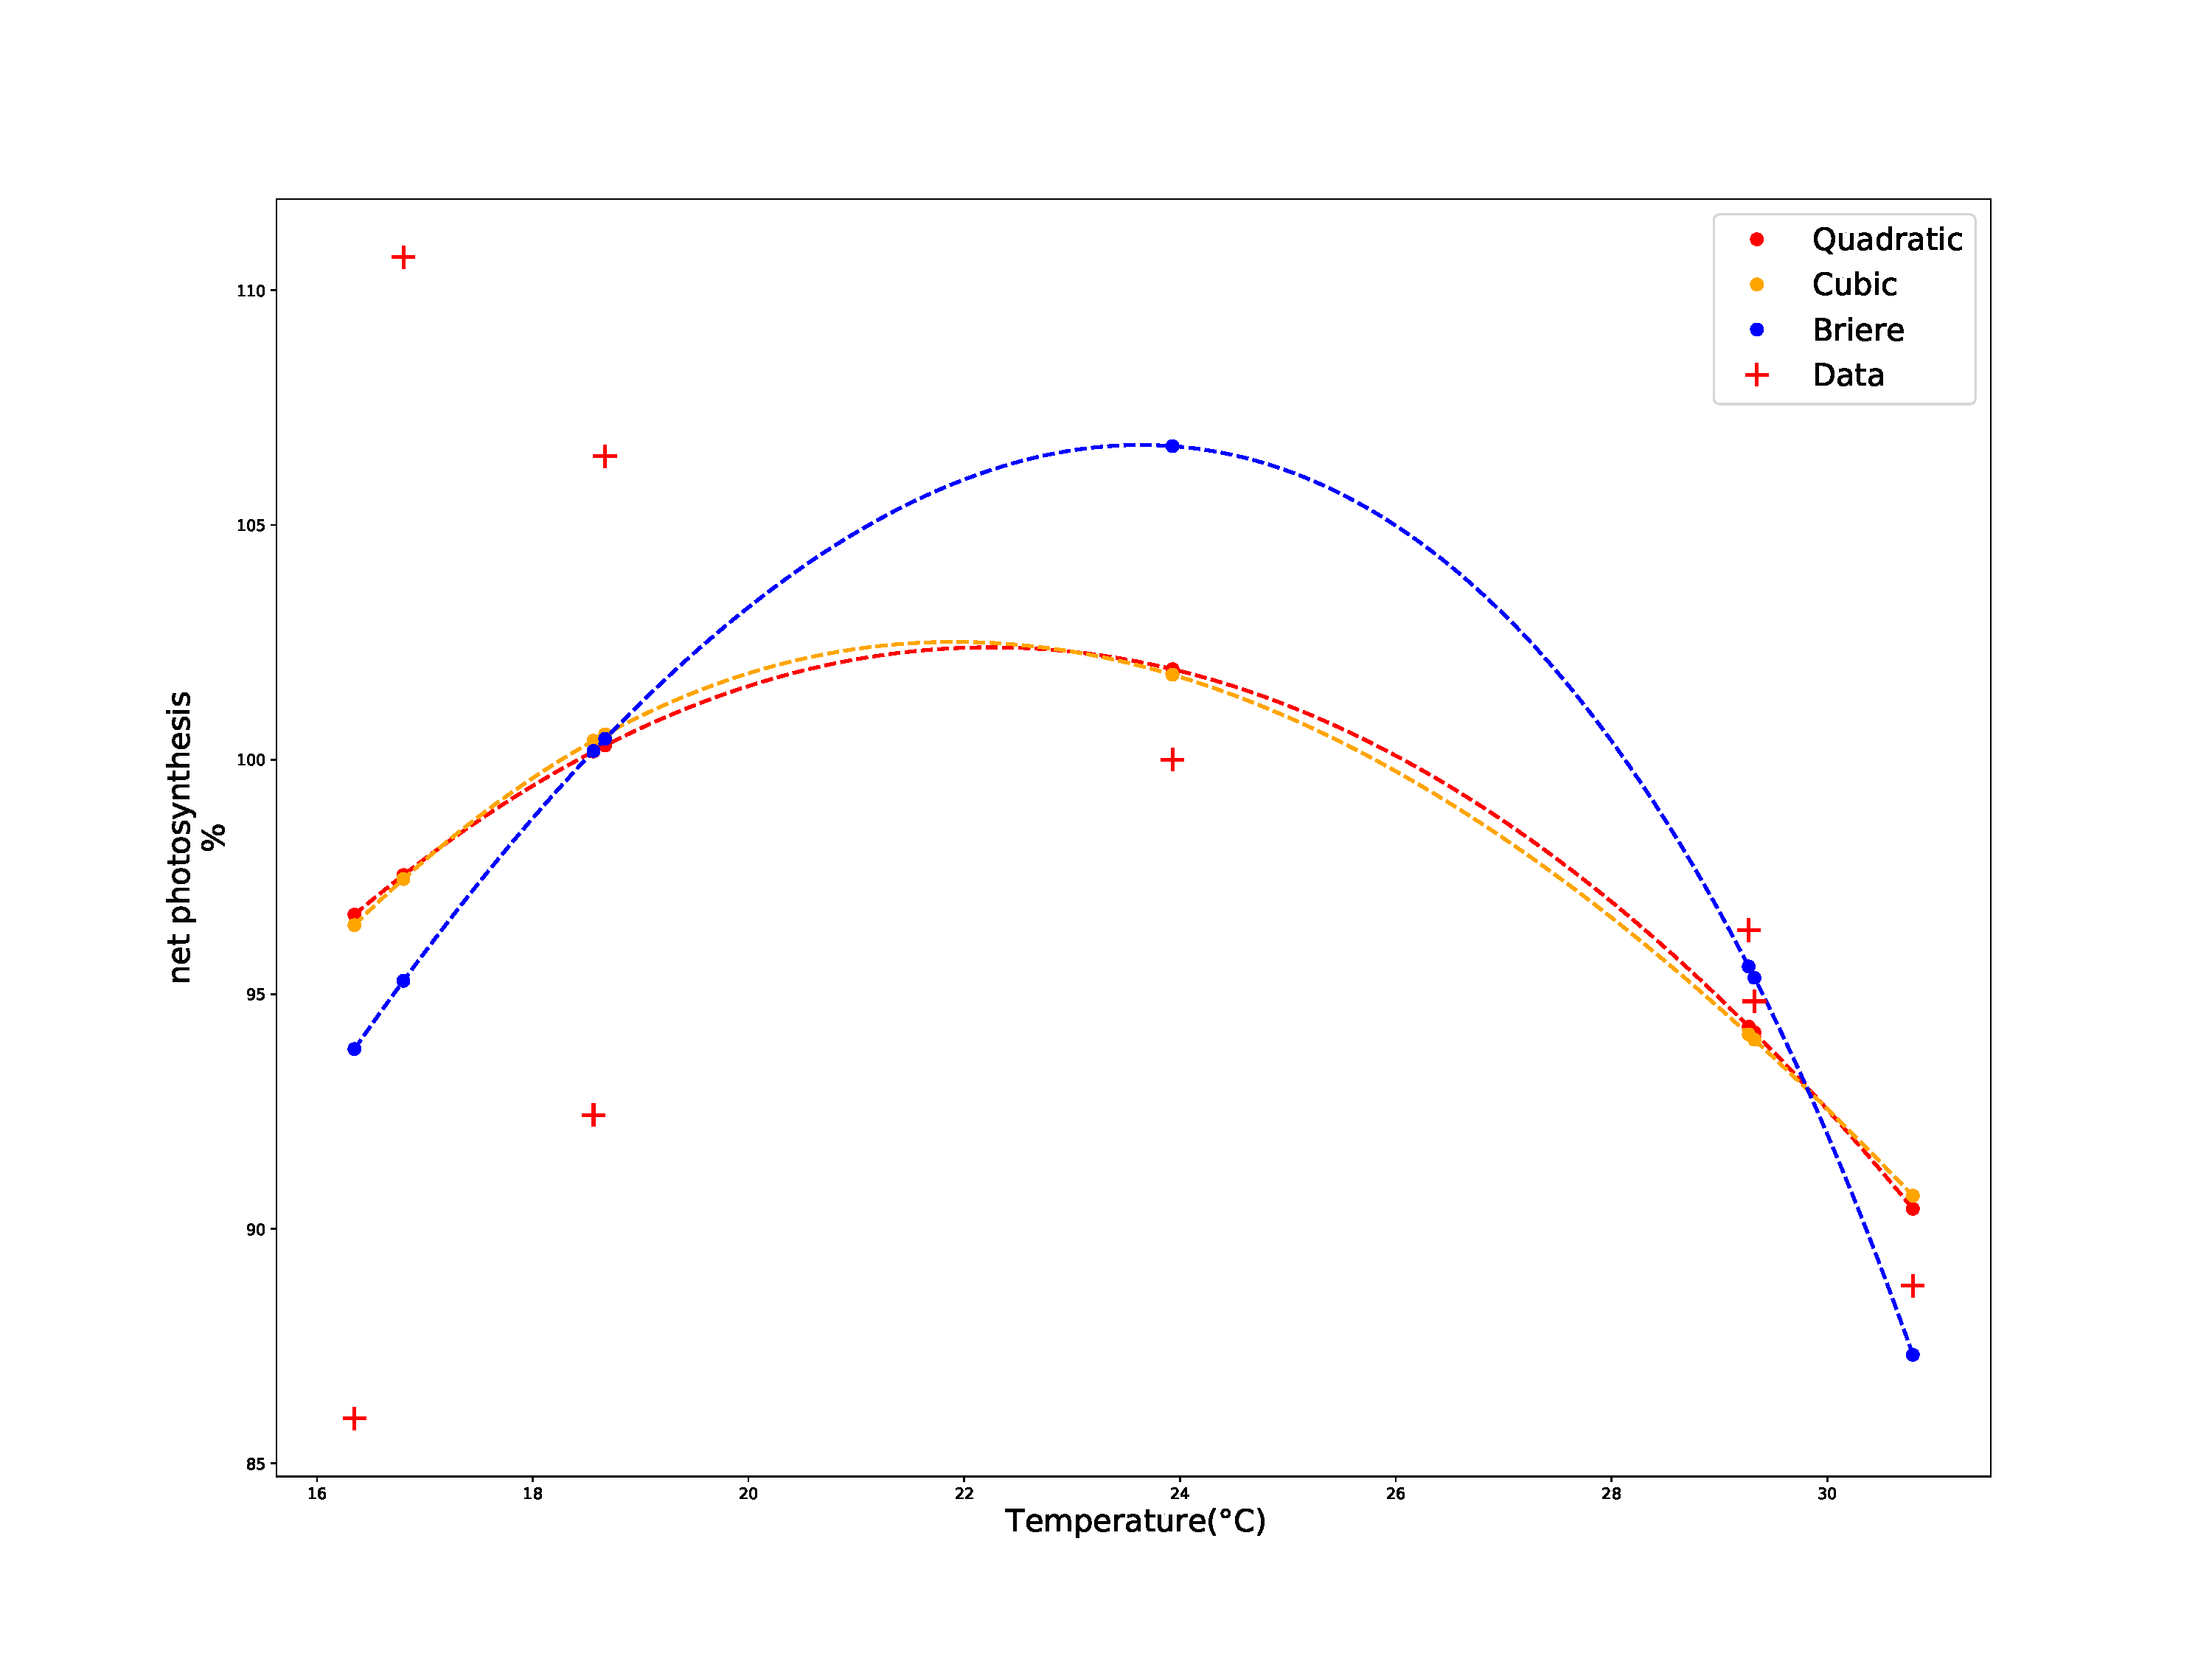
\includegraphics[width=\linewidth]{images/TPC_fitting511.pdf}
      \caption{\textbf{ID:511}}
    \end{subfigure}
    \hfill
    \begin{subfigure}[t]{.5\textwidth}
      \center
      \includegraphics[width=\linewidth]{images/TPC_fitting519.pdf}
      \caption{\textbf{ID:519}}
    \end{subfigure}
  
    \medskip

  % \hspace*{-1cm}
    \begin{subfigure}[t]{.5\textwidth}
      \center
      \includegraphics[width=\linewidth]{images/TPC_fitting568.pdf}
      \caption{\textbf{ID: 568}}
    \end{subfigure}
    \hfill
    \begin{subfigure}[t]{.5\textwidth}
    \center
      \includegraphics[width=\linewidth]{images/TPC_fitting600.pdf}
      \caption{\textbf{ID: 600}}
    \end{subfigure}
    \caption{Datasets that have poor fitting of mechanistic model}
  \end{figure}

  From the results shown above, there is no significant difference in model assessment between the AIC approach and BIC approach. The rank of the best-fit model is not affected, although a little gap can be seen for each model as different approaches of model assessment apply.  Also, the trend is similar to the most datasets when distinct rules apply except for the dataset of photosynthesis, where a significant differences between model performance of cubic model can be seen as applying different rules.

  Due to the interpretability of the mechanistic model, it is expected to be have better performance than some phenomenological or statistical models. However, it is not always true in the project, where the simplified Schoolfield model was the best model only in the photosynthesis dataset when applying rule of single model selection. The reason for this may the mechanistic models have more restrict hypotheses than phenomenological ones, which results in the fitting of mechanistic model is invalid. The figure 3 showed some examples of failed or poor fittings of individual datasets. 

  By comparison, AIC and BIC both provided similar outcomes and model selection, although there may be a little differences between results of them. Thus, any one of them can be selected as a main model assessment method in my project. However, AIC was preferred to use in this project. The reasion is (1) AIC is a suitable approach for sparse datasets, given that it is an estimator derived from basic thoery called K-L information theory, which is possible for further correction.Thus, this leads AIC to have second-order derived version that can deliminate estimated bias of small sample size \cite{burnham_anderson_2004}. (2) BIC expects the "true model" to be in the model set while AIC does not \cite{johnson_2004}.

  The motivation of the project is to analyse four candidate models and provide a reasonable comparison between them. However, there are also more works need to be done. Firstly, the starting values of two non-linear models are selected by normal distribution sampling method, which may be not enough for finding the precise starting values. Thus, this may be also the reason why linear model outperformed non-linear model in respiration dataset. A better approach to find the starting value of parameters for non-linear models should be implemented. Secondly, only one mechanistic model are used to make a model comparison here, may causing bias of the results. Thus, more mechanistic models are worthy of consideration in order to improve the accuracy of the results. Third, due to limited computational power, only approximately maximum 300 repeats of fitting for each indivial dataset is available. Hence, more repeats are suppose to be attempted for obtaining more accurate outcome if the computer with stronger computational power is available such as high-performance computer or other supercomputers.

\section{Conclusion}

In conclusion, the mechanistic model, simplified Schoolfield, is significantly useful when fitting the data of biological rate since the data pattern of approximately 42\% of dataset was captured, although cubic model outperformed it in some cases. However, the simplified Schoolfield model does not show an obvious advantage when fitting the datasets of respiration rate, due to the data specificity and strictness of assumptions of mechanistic models. Therefore, there is no sufficient evidence that can conclude that mechanistic model is better than phenomenological models. To select the best models between them, if possible, all datasets should be considered case by case.

\bibliographystyle{plain}
\bibliography{references}


% \section{Appendices}
\end{document}} % Supervisor's Name
    
    %----------------------------------------------------------------------------------------
    %	LOGO SECTION
    %----------------------------------------------------------------------------------------
    
    
\includegraphics[width=7cm]{../Results/Results_backup/images/logo.eps}\\[1cm] 
    % Include a department/university logo - this will require the graphicx package
     
    %----------------------------------------------------------------------------------------
    
    \center % Center everything on the page
    
    %----------------------------------------------------------------------------------------
    %	HEADING SECTIONS
    %----------------------------------------------------------------------------------------
    
    % \textsc{\LARGE MSc Computational Methods in Ecology and Evolution}\\[1.5cm] % Name of your university/college
    \textbf{\large Imperial College London}\\[0.8 cm] % Major heading such as course name
    \textbf{\large Department of Life Sciences, Faculty of Natural Sciences}\\[0.8 cm] % Minor heading such as course title
    %----------------------------------------------------------------------------------------
    %	TITLE SECTION
    %----------------------------------------------------------------------------------------
    \makeatletter
    \HRule \\[0.6cm]
    { \huge \bfseries \@title}\\[0.6cm] % Title of your document
    \HRule \\[1.5cm]

    \begin{minipage}{0.4\textwidth}
      \begin{flushleft} \large
      \emph{Author:}\\
      Jingkai \textsc{SUN} \\[0.5cm]
      \emph{CID:}\\
      01991822
      \end{flushleft}
      \end{minipage}
      ~
      \begin{minipage}{0.5\textwidth}
      \begin{flushright} \large
      \emph{Date:} \\
      \today \\[0.5cm] % Supervisor's Name
      \emph{Word Count:} \\
      \wordcount


      \end{flushright}
    \end{minipage}\\[1cm]
 
 
    % \center
    % \textbf{\huge Word Count: 2065}
    
    \vfill % Fill the rest of the page with whitespace
    
    \end{titlepage}

\maketitle
\linenumbers

\begin{abstract}
The photosynthesis and respiration rate are essential biological traits of organisms, they are all responsed to their body temperature, indicating that creating effective mathematical model to describe them is becoming increasingly crucial. This project has used four candidate models (Quadratic, Cubic, Briere and simplified Schoolfield models), where quadratic, cubic and briere are phenomenological models and simplified Schoolfield is mechanistic model, to fit 378 datasets of photosynthesis rate and 249 datasets of respiration rate grouped by different IDs of organisms. The result shows that simplified Schoolfield model is effective for fitting datasets of photosynthesis rate, although cubic may be better than it in some cases.
\end{abstract}


\section{Introduction}

Thermal performance curve (TPC) describes the relationship between biological traits (e.g. photosynthesis, respiration and growth rate) and temperature, which is an essential factor in ecology, biology and physiology \cite{huey_1989}. Due to the importance of TPC, numerous biological temperature-dependent rate models have been implemented, it has been increasingly important that using computer tools to fit the model \cite{angilletta_2002}, many authors have taken advantages of programming language for model fitting in their paper. However, the paper concerning the comparison between published models is scarce. Therefore, this project aims at giving a comparison between distinct models fitting the thermal performance curve. The remaining sections in this report will be explained as follow. In section 2, a brief introduction of candidate models and an explanation of data preprocessing will be given, then I will explain the method and assessment tool used. In section 3, the results of the fitted model will be explained. Next section will give a conclusion for the results and some future works that can be done.

\section{Experimental Data and Fitting Methods}

\subsection{Experimental Data}

The part of ”BioTraits” database, containing 903 fitted subsets, was selected as the main research object for the model analysis with columns (”ID”, ”ConTemp(°C)”, ”OriginalTraitValue”, ”StandardisedTraitName”). Some preprocess had been done to the original dataset. Firstly, all observations where the Original Trait Value is less than or equal to zero had been removed for logarithm purpose. Then, to obtain more reasonable curves, all datasets in which data points are less than or equal to 5 (276 out of 903) were deleted. Afterwards, the datasets were divided into two subsets based on the ”StandardisedTraitName”, which is ”photosynthesis rate” and ”respiration rate”. Then, there were 378 and 249 (627 subsets in total) subsets in two datasets with different biological traits respectively.

\subsection{Candidate Models}

Four models were chosen in this project, including two linear models (Quadratic and Cubic) and two non-linear models (Briere and Schoolfield Model with High-Temperature Term). For two linear and Briere models, they are phenomenological models lacking some biological interpretation, while Schoolfield is a mechanistic model that has some biological meaning behind that. Briere (1) and Schoolfield (2) model have mathematical expressions as follow:

\begin{equation}
    B =
    \begin{cases}
    0,                           &\text{$T \leq T_0$} \\
    B_0T(T-T_0) \sqrt {T_m - T}, &\text{$T_0 \leq T \leq T_m$} \\
    0,                           &\text{$T \geq T_m$}
    \end{cases}
\end{equation}

where B is biological trait, which is a function of temperature T. $T_l$ is the maximum temperature that organisms can bear.
$T_0$ is the lowest temperature threshold, and B0 is the empirical constant. There are some assumptions for fitting the data well \cite{briere_pracros_1999}.

\begin{itemize}
    \item It is possible to adjust the muximum or minimum thresholds of temperature \cite{briere_pracros_1999}. 
    \item Asymmetric shape around peak temperature ($T_{opt}$) \cite{briere_pracros_1999}.
    \item There is a sharp drop after passing the $T_{opt}$ \cite{briere_pracros_1999}.
    \item There is an inflection point in the datasets \cite{briere_pracros_1999}.
\end{itemize}

The full Schoolfield model is expressed as follows \cite{SCHOOLFIELD1981719}:
\begin{equation}
    B = B_0 \frac { e^{\frac{-E_a}{k}(\frac{1}{T} - \frac{1}{283.5})} }
                { 1 + e^{\frac{E_l}{k}(\frac{1}{T_l} - \frac{1}{T})} + 
                e^{\frac{E_h}{k} (\frac{1}{T_h} - \frac{1}{T}) }}
\end{equation}

where k is Boltzmann constant, B is the biological rate responsed by temperature T in Kelvin unit. $B_0$ is the biological rate at low temperature. $E_a$ is the activation energy that determine the increase in temperature up to the optimum. $E_l$ 
is the de-activation energy at low temperature. $T_l$ is the low temperature that enzyme is 50\% de-activated. $E_h$ is the de-activation energy at high temperature, while $T_h$ is temperature at which the enzyme is 50\% high-temperature deactivated.
However, it is difficult to detect the low-temperature deactivation energy \cite{kontopoulos_2018}. Thus, the schoolfield with only high temperature term (eq.3) was used in this porject:

\begin{equation}
    B = B_0 \frac { e^{\frac{-E_a}{k}(\frac{1}{T} - \frac{1}{283.5})} }
                { 1 + e^{\frac{E_h}{k} (\frac{1}{T_h} - \frac{1}{T}) }}
\end{equation}

To capture the data pattern more precisely, the Schoolfield equation is rewritten as logarithmic form:

\begin{equation}
    ln(B) = ln(B_0) - \frac{E_a}{k} \times (\frac{1}{T} - \frac{1}{283.5}) - ln(1 + e^{\frac{E_h}{k} (\frac{1}{T_h} - \frac{1}{T}) })
\end{equation}

With simplified Schoolfield model, some assumptions are also needed to capture the data pattern well \cite{delong_2017}:

\begin{itemize}
    \item All traits (biological rates) is controlled by single enzyme \cite{delong_2017}
    \item enzymes need to be deactivated at high temperature \cite{delong_2017}
    \item the activation energy ($E_a$) corresponds to the optimal enzyme activity level \cite{delong_2017}
\end{itemize}

In addition, this project also assumes that there is no interation terms between linear models.

\subsection{Model Assessment}

All four candidate models mentioned above were assessed. The starting values of two non-linear models were found as follow:
For Briere model, the maximum and minimum temperature is given by parameters $T_m$ and $T_0$ respectively. Initial $B_0$ is chosen to be 0.01 manually. For simplified Schoolfield model, initial $B_0$ is just the biological rate at the lowest temperature. $E_a$ and  $E_h$ are selected to be the absolute values of slope and slope times ten by running the logarithmic Arrhenius model respectively.  Finally, the temperature (or the average of the temperature if there more than two values) that has the highest rate is given to the initial $T_h$. After assigning initial values, the starting value will be chosen randomly using normal distribution method with mean as the value of parameters as well as appropriate bounding and standard deviation values, the fitted data such as TSS, RSS, $R^2$, AIC and BIC are calculated. The whole fitting process will be repeated by a minimum 200 and maximum of 300 rounds in order to find the best fit with the lowest AIC value.

Akaike Information Criterion (AIC) and Bayesian Information Criterion (BIC) were calculated for model analysis. These metrics allow us to choose which model performs the best. The AIC approach is an information-theoretic selection by calculating Kullback-Leibler (K-L) distance \cite{burnham_anderson_2004} \cite{burnham_anderson2010}, while the BIC method is based on Bayes factors. All those values are expected to be the lower, the better. However, these metrics will cause the issue if they are used independently since they are used to compare with other values, there is no point computing AIC vlaue for single model. \cite{guthery_2003}. Thus, the AIC differences were also calculated in order to rank models and include more reasonable best-fit models. The rule of thumb of AIC differences allows us to consider more models as the best-fit model for each trial if the value differences between two models are less than 2, expressed as $ \Delta AIC_i/BIC_i < 2$ \cite{burnham_anderson2010}.


\subsection{Computing Tools}

In this project, Python 3 with packages "lmfit", "numpy", "pandas" and "matplotlib" was used as the main tool of creating model fitting program. R (4.0.3) with packages "dplyr" and "ggplot2" was used to analyse and visualise the fitted information of each model obtained after the model fitting program is done. Python 3 with package "subprocess" and "os" was used to integrate all project scripts.

\section{Results}
% Figures of total counts
\begin{figure}[H]
    \centering
    \includegraphics[width = 15cm, height = 12cm]{../Results/Results_backup/images/bestfit_total_rule2.pdf}
    \caption{Best fit occurrence using rule of $\Delta AIC/BIC + 2$}
\end{figure}

Figure 1 gives the best-fit occurrence for each models using AIC or BIC difference rule. Surprisingly, cubic has the most outstanding performance compared with all other models. However, simplified Schoolfield, the only mechanistic model in candidate ones, has the second most times becoming the best fit model. Cubic is the best model of 387 datasets (based on AIC assessment) and 337 datasets (based on BIC assessment) out of 627 datasets, accounting for approximately 67\% and 58\% of total datasets respectively, while simplified Schoolfield is the best model of 245 and 237 datasets based on different measurement metrics, accounting for 42\% and 41\% of the total. Also, 108 datasets have both cubic and Schoolfield models as best fit models based on the rule of AIC/BIC differences. For the remaining two models, quadratic became the best-fit model of 198 and 201 datasets according to AIC and BIC values, which is 34 and 33 datasets more than Briere. 

\begin{figure}[H]
    % \hspace*{-1cm}
    \center
    \includegraphics[height = 14cm, width = 15cm]{../Results/Results_backup/images/bestfit_grouped_rule2.pdf}
    \caption{Best-Fit Occurence Based on Different Datasets and Assessment Methods}
\end{figure}

Figure 2 illustrates the number of best-fit models in datasets of photosynthesis and respiration rate using AIC or BIC difference and the method of single model selection with the lowest AIC/BIC values. First of all, with using the AIC/BIC difference approach to count best models, two datasets showed very different results. For the dataset of photosynthesis, furthermore, cubic and simplified Schoolfield are also the top 2 models that have the highest counts of the best fit. Cubic is the best-fit model of 191 datasets of fitting out of 335 datasets, which is 29 datasets more than the simplified Schoolfield using AIC approach but only 7 more by BIC approach, while there is no significant difference between quadratic and Briere models. In respiration datasets, cubic is still the winner compared other models, becoming the best-fit model in 81\% or 70\% of the total by distinct model assessment approaches. However, quadratic became the second best-fit model, taking the place of the simplified Schoolfield model. By choosing the single model with lowest AIC/BIC values in each trial, interestingly, the simplified Schoolfield model beats all other three models, being the best model in 35\% - 36\% of total photosynthesis data, while cubic and quadratic models still outperform other ones in the dataset of respiration rate.

\section{Discussion}

\begin{figure}
    \begin{subfigure}[t]{.5\textwidth}
      \center
      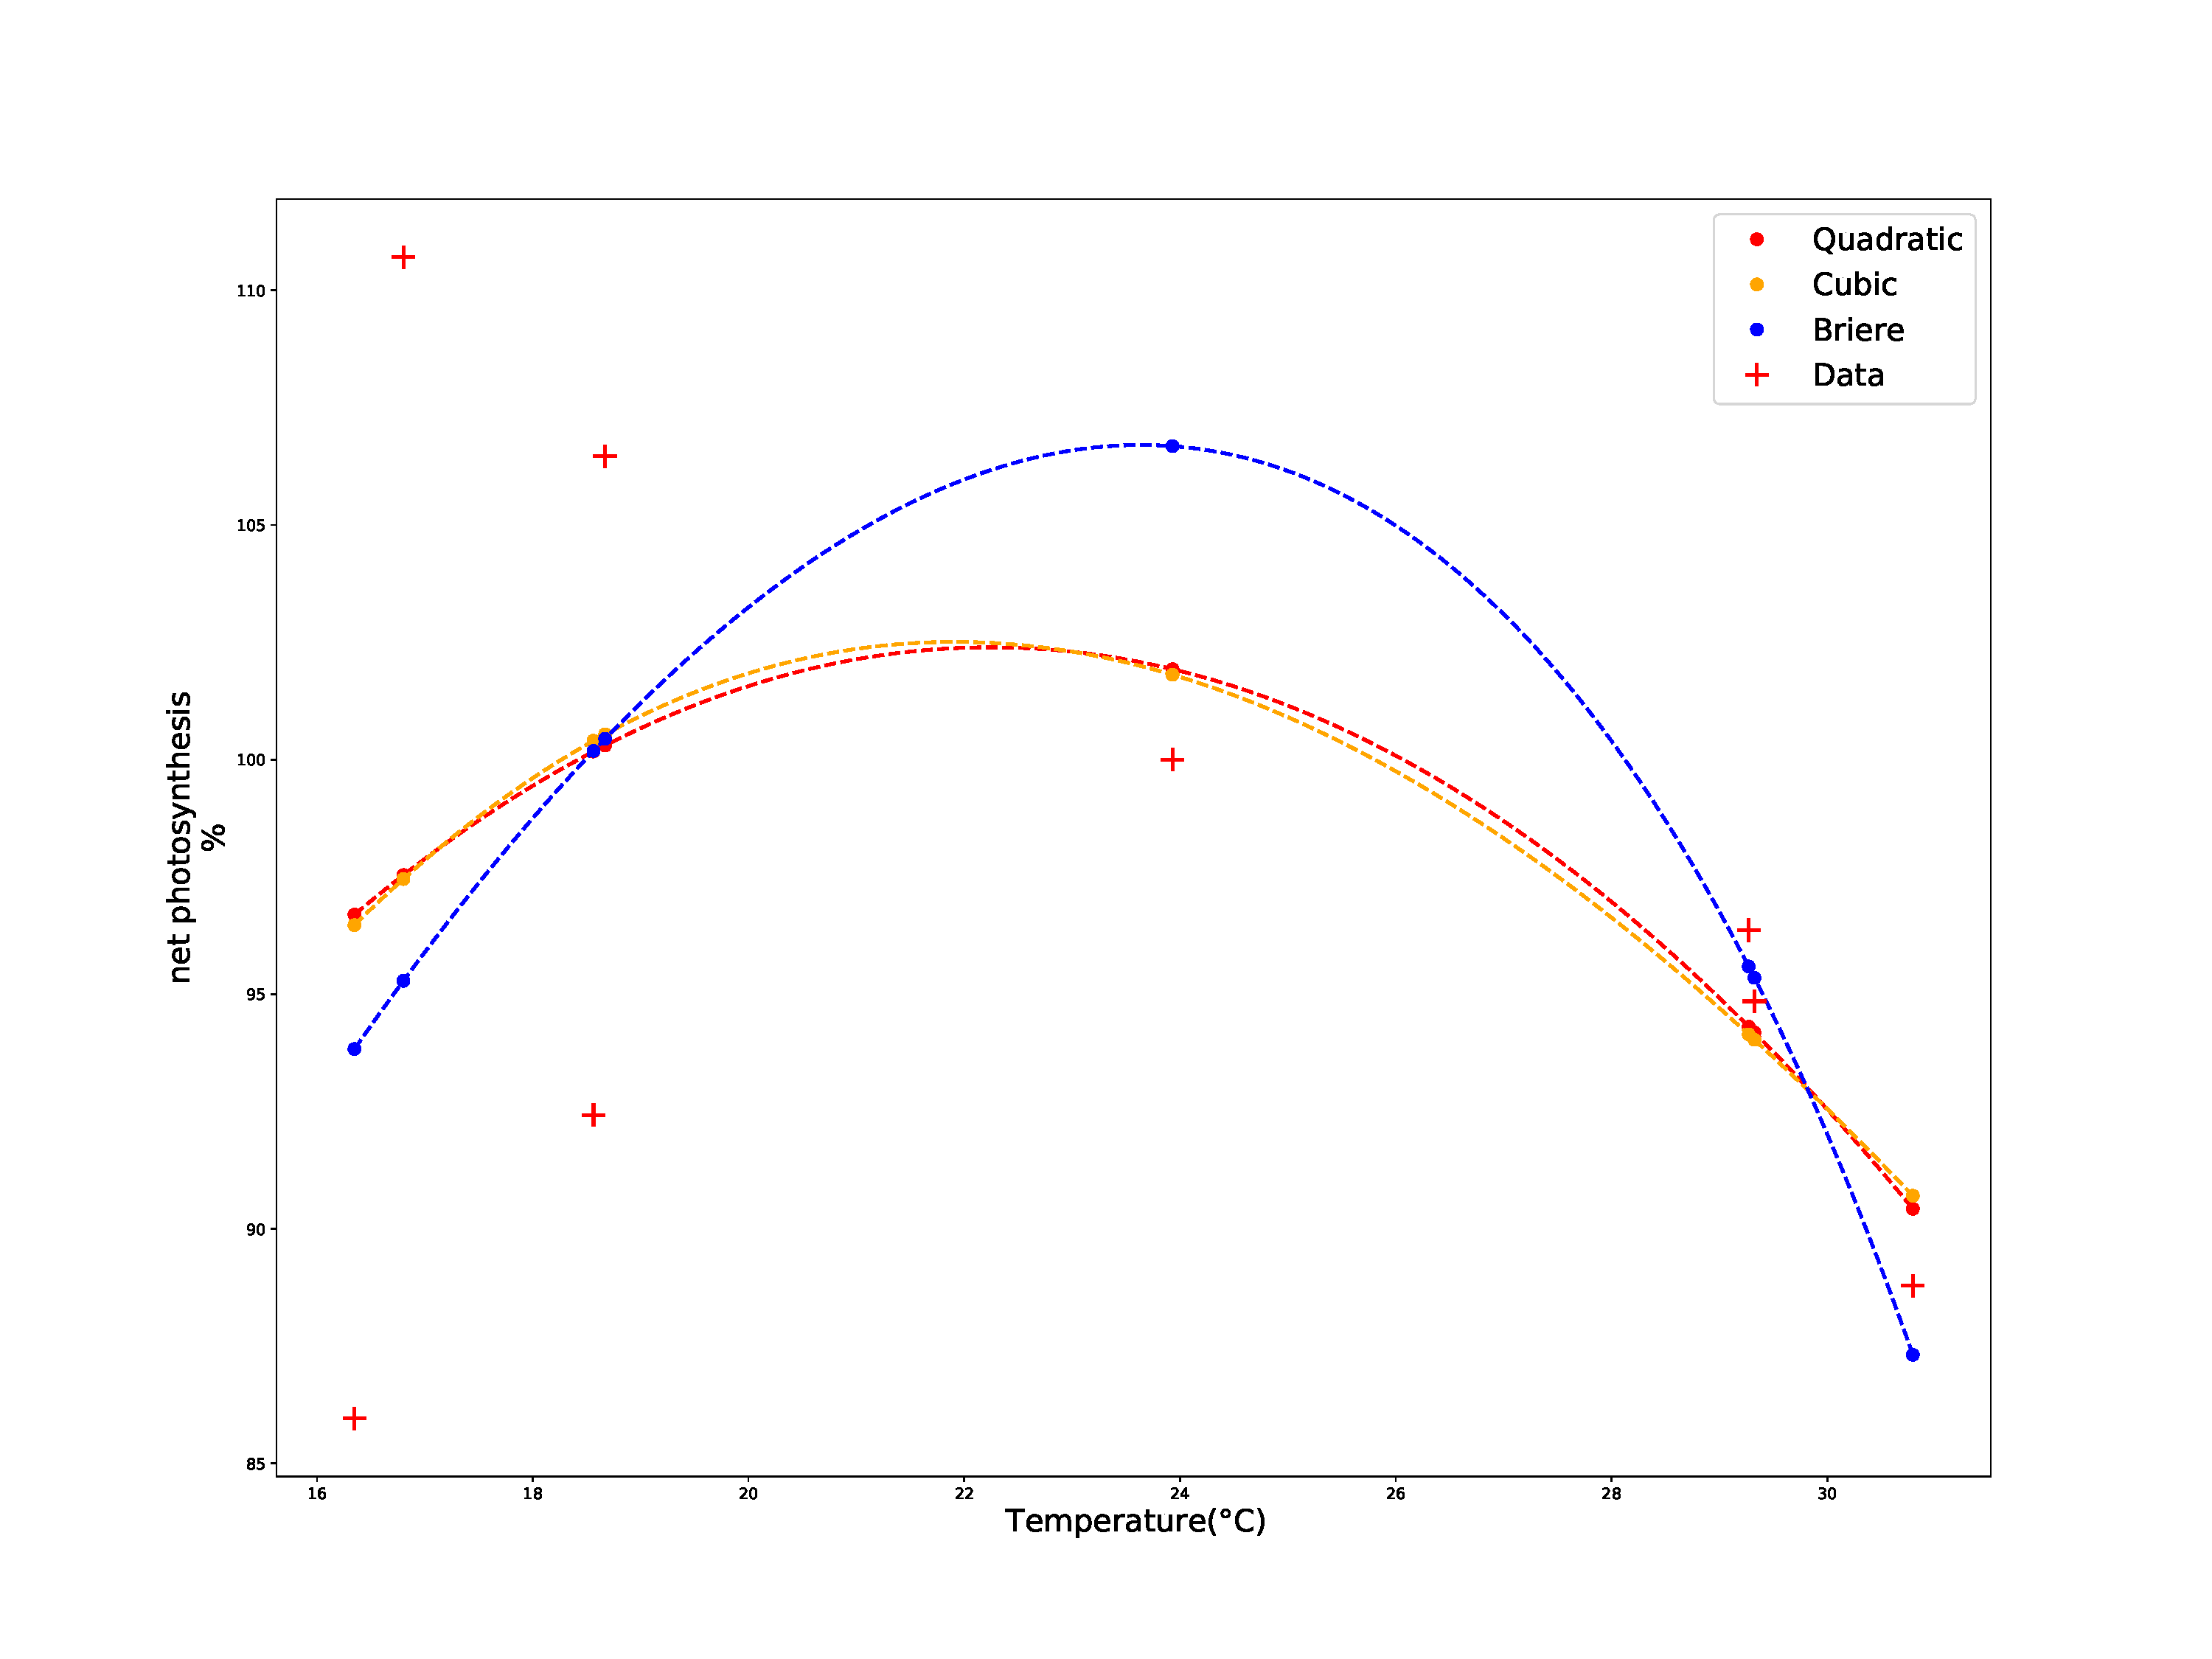
\includegraphics[width=\linewidth]{../Results/Results_backup/images/TPC_fitting511.pdf}
      \caption{\textbf{ID:511}}
    \end{subfigure}
    \hfill
    \begin{subfigure}[t]{.5\textwidth}
      \center
      \includegraphics[width=\linewidth]{../Results/Results_backup/images/TPC_fitting519.pdf}
      \caption{\textbf{ID:519}}
    \end{subfigure}
  
    \medskip

  % \hspace*{-1cm}
    \begin{subfigure}[t]{.5\textwidth}
      \center
      \includegraphics[width=\linewidth]{../Results/Results_backup/images/TPC_fitting568.pdf}
      \caption{\textbf{ID: 568}}
    \end{subfigure}
    \hfill
    \begin{subfigure}[t]{.5\textwidth}
    \center
      \includegraphics[width=\linewidth]{../Results/Results_backup/images/TPC_fitting600.pdf}
      \caption{\textbf{ID: 600}}
    \end{subfigure}
    \caption{Datasets that have poor fitting of mechanistic model}
  \end{figure}

  From the results shown above, there is no significant difference in model assessment between the AIC approach and BIC approach. The rank of the best-fit model is not affected, although a little gap can be seen for each model as different approaches of model assessment apply.  Also, the trend is similar to the most datasets when distinct rules apply except for the dataset of photosynthesis, where a significant differences between model performance of cubic model can be seen as applying different rules.

  Due to the interpretability of the mechanistic model, it is expected to be have better performance than some phenomenological or statistical models. However, it is not always true in the project, where the simplified Schoolfield model was the best model only in the photosynthesis dataset when applying rule of single model selection. The reason for this may the mechanistic models have more restrict hypotheses than phenomenological ones, which results in the fitting of mechanistic model is invalid. The figure 3 showed some examples of failed or poor fittings of individual datasets. 

  By comparison, AIC and BIC both provided similar outcomes and model selection, although there may be a little differences between results of them. Thus, any one of them can be selected as a main model assessment method in my project. However, AIC was preferred to use in this project. The reasion is (1) AIC is a suitable approach for sparse datasets, given that it is an estimator derived from basic thoery called K-L information theory, which is possible for further correction.Thus, this leads AIC to have second-order derived version that can deliminate estimated bias of small sample size \cite{burnham_anderson_2004}. (2) BIC expects the "true model" to be in the model set while AIC does not \cite{johnson_2004}.

  The motivation of the project is to analyse four candidate models and provide a reasonable comparison between them. However, there are also more works need to be done. Firstly, the starting values of two non-linear models are selected by normal distribution sampling method, which may be not enough for finding the precise starting values. Thus, this may be also the reason why linear model outperformed non-linear model in respiration dataset. A better approach to find the starting value of parameters for non-linear models should be implemented. Secondly, only one mechanistic model are used to make a model comparison here, may causing bias of the results. Thus, more mechanistic models are worthy of consideration in order to improve the accuracy of the results. Third, due to limited computational power, only approximately maximum 300 repeats of fitting for each indivial dataset is available. Hence, more repeats are suppose to be attempted for obtaining more accurate outcome if the computer with stronger computational power is available such as high-performance computer or other supercomputers.

\section{Conclusion}

In conclusion, the mechanistic model, simplified Schoolfield, is significantly useful when fitting the data of biological rate since the data pattern of approximately 42\% of dataset was captured, although cubic model outperformed it in some cases. However, the simplified Schoolfield model does not show an obvious advantage when fitting the datasets of respiration rate, due to the data specificity and strictness of assumptions of mechanistic models. Therefore, there is no sufficient evidence that can conclude that mechanistic model is better than phenomenological models. To select the best models between them, if possible, all datasets should be considered case by case.

\bibliographystyle{plain}
\bibliography{references}


% \section{Appendices}
\end{document}